\documentclass[compress]{beamer}
\usepackage{graphicx,amsmath,amsthm,verbatim,bm}
\usepackage{longtable}
%\usetheme{Copenhagen}
%\useoutertheme[{options}]{tree}
%\setbeamertemplate{footline}[page number]
%\useoutertheme{infolines}
%\setbeamertem plate{headlirne}{}
\useinnertheme{circles}
\usepackage{comment}
\setbeamertemplate{footline}[frame number]
%\usepackage{times}
%\usepackage[tbtags]{amsmath}
%\usepackage{amssymb}
\usepackage{amsfonts}
%\usepackage{slfortheorems}
\usepackage{epsfig}
\usepackage{graphicx}
\usepackage[small]{caption}
\usepackage[square]{natbib}
%\newcommand{\newblock}{}
\bibpunct{(}{)}{;}{a}{}{,}
\bibliographystyle{ims}
%\usepackage[letterpaper]{geometry}
\usepackage{color}
\setlength{\parindent}{0pt}
\usepackage{bbding}
\usepackage{long table, booktabs}



\usepackage{listings}
\usepackage[ruled,lined]{algorithm2e}
\def\algorithmautorefname{Algorithm}
\SetKwIF{If}{ElseIf}{Else}{if}{then}{else if}{else}{endif}

\usepackage{longtable}



\theoremstyle{plain}
\usepackage{amsfonts}
\usepackage{epsfig}
\usepackage{graphicx}
%\usepackage[small]{caption}

\usepackage{zref-savepos}

\newcounter{restofframe}
\newsavebox{\restofframebox}
\newlength{\mylowermargin}
\setlength{\mylowermargin}{2pt}

\newenvironment{restofframe}{%
    \par%\centering
    \stepcounter{restofframe}%
    \zsavepos{restofframe-\arabic{restofframe}-begin}%
    \begin{lrbox}{\restofframebox}%
}{%
    \end{lrbox}%
    \setkeys{Gin}{keepaspectratio}%
    \raisebox{\dimexpr-\height+\ht\strutbox\relax}[0pt][0pt]{%
    \resizebox*{!}{\dimexpr\zposy{restofframe-\arabic{restofframe}-begin}sp-\zposy{restofframe-\arabic{restofframe}-end}sp-\mylowermargin\relax}%
        {\usebox{\restofframebox}}%
    }%
    \vskip0pt plus 1filll\relax
    \mbox{\zsavepos{restofframe-\arabic{restofframe}-end}}%
    \par
}


\usepackage{tikz}
\usetikzlibrary{arrows}

%\usepackage[usenames,dvipsnames]{xcolor}
\usepackage{tkz-berge}
\usetikzlibrary{fit,shapes}

\usepackage{calc}
\usetikzlibrary{decorations.markings}

\tikzstyle{vertex}=[circle, draw, inner sep=0pt, minimum size=6pt]
\newcommand{\vertex}{\node[vertex]}
\newcounter{Angle}



%%%to add in new counter for slides in beamer
\newcommand{\beginbackup}{
   \newcounter{framenumbervorappendix}
   \setcounter{framenumbervorappendix}{\value{framenumber}}
}
\newcommand{\backupend}{
   \addtocounter{framenumbervorappendix}{-\value{framenumber}}
   \addtocounter{framenumber}{\value{framenumbervorappendix}} 
}


\newcommand*\oldmacro{}
\let\oldmacro\insertshortauthor
\renewcommand*\insertshortauthor{
  \leftskip=.3cm
\insertframenumber\,/\,\inserttotalframenumber\hfill\oldmacro}




\excludecomment{notbeamer}
\includecomment{beamer}

\newcommand{\lam}{\mathbf{\Lambda}}	
\newcommand{\bX}{\mathbf{X}}
\newcommand{\bY}{\mathbf{Y}}

\title[ Entity Resolution with Societal Impacts in Statistical Machine Learning]
{ Entity Resolution with Societal Impacts in Statistical Machine Learning}
\author[Beidi Chen and Rebecca C. Steorts, beka@stat.duke.edu]{Beidi Chen and Rebecca C. Steorts} 

\institute{\normalsize Rice University, Department of Computer Science \\Department of Statistical Science, affiliated faculty in Computer Science, Biostatistics and Bioinformatics, the information initiative at Duke (iiD) and \\the Social Science Research Institute (SSRI) \\ Duke University and U.S. Census Bureau\\ \vspace*{0.2em}

\begin{figure}[htbp]
\begin{center}

\includegraphics{figures/banner}
%\caption{default}
\label{default}
\end{center}
\end{figure}}
\date{February 8, 2017}


\begin{document}
\begin{frame}
\titlepage
\end{frame}



\frame{

\begin{itemize}
\frametitle{Summary}
\pause
\item Entity resolution: merging large, noisy databases.
\pause
\begin{itemize}
\item Medical data, official statistics, genetic data, human rights violations, and more. \ldots
\end{itemize}
\pause
\item In human rights, and more specifically 
in studies of conflict violence, we rarely 
have access to complete data.
\pause
\begin{itemize}
\item Instead, we have snapshots 
of violence and killings.

\end{itemize}
\pause

\item Seek important questions about human rights killings that  use  \textcolor{blue}{sound statistical} and \textcolor{blue}{machine learning} techniques. 
\pause
\begin{itemize}
\item We wish to quantify the number of documented identifiable deaths in the Syrian conflict and quantify a standard error.  
\pause
\item We propose a statistical learning approach that is much less than quadratic, allowing computational efficiency.  
\pause
\item We do not make any distributional assumptions about the data generating process. 
\pause
\item Our proposed estimator is unbiased and has provably low variance compared to the current literature. 
\pause
\item We illustrate our methodology on a subset of the Syrian conflict, which closely matches that from the 2014 Human Rights Data Analysis Group (HRDAG).
\end{itemize}
%\begin{itemize}
%
%\end{itemize}



\end{itemize}


}



%\begin{frame}
%\frametitle{Motivations}
%  \begin{columns}[T]
%    \begin{column}{.5\textwidth}
%     \begin{block}{In Syria, we have duplicated information regarding individuals who have died in the conflict. \\
%\vspace*{2em}
%   In the census, we have duplicated information of individuals that fill out census forms every 10 years. \\
%\vspace*{2em}
%Goal: Estimation of the sample size and associated standard errors. 
% }
%% Your text here
%    \end{block}
%    \end{column}
%    \begin{column}{.5\textwidth}
%    \begin{block}{}
%% Your image included here
%    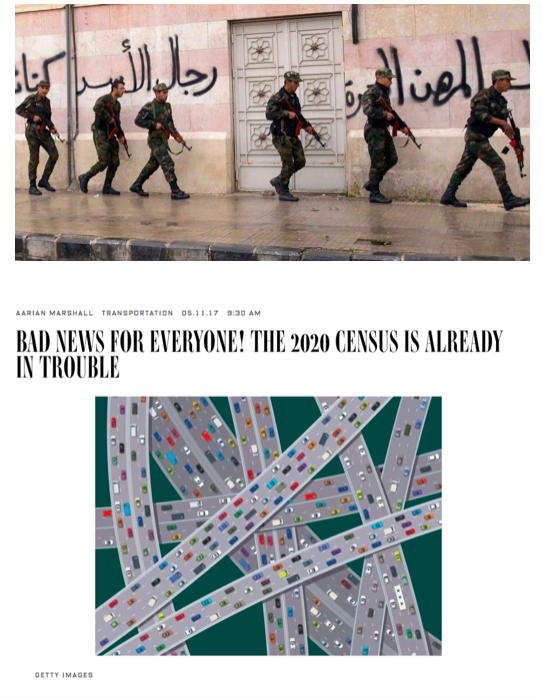
\includegraphics[width=\textwidth]{syria-census2}
%    \end{block}
%    \end{column}
%  \end{columns}
%\end{frame}


\frame{


\begin{figure}[htbp]
\frametitle{Do we already know the answer?}
\begin{center}
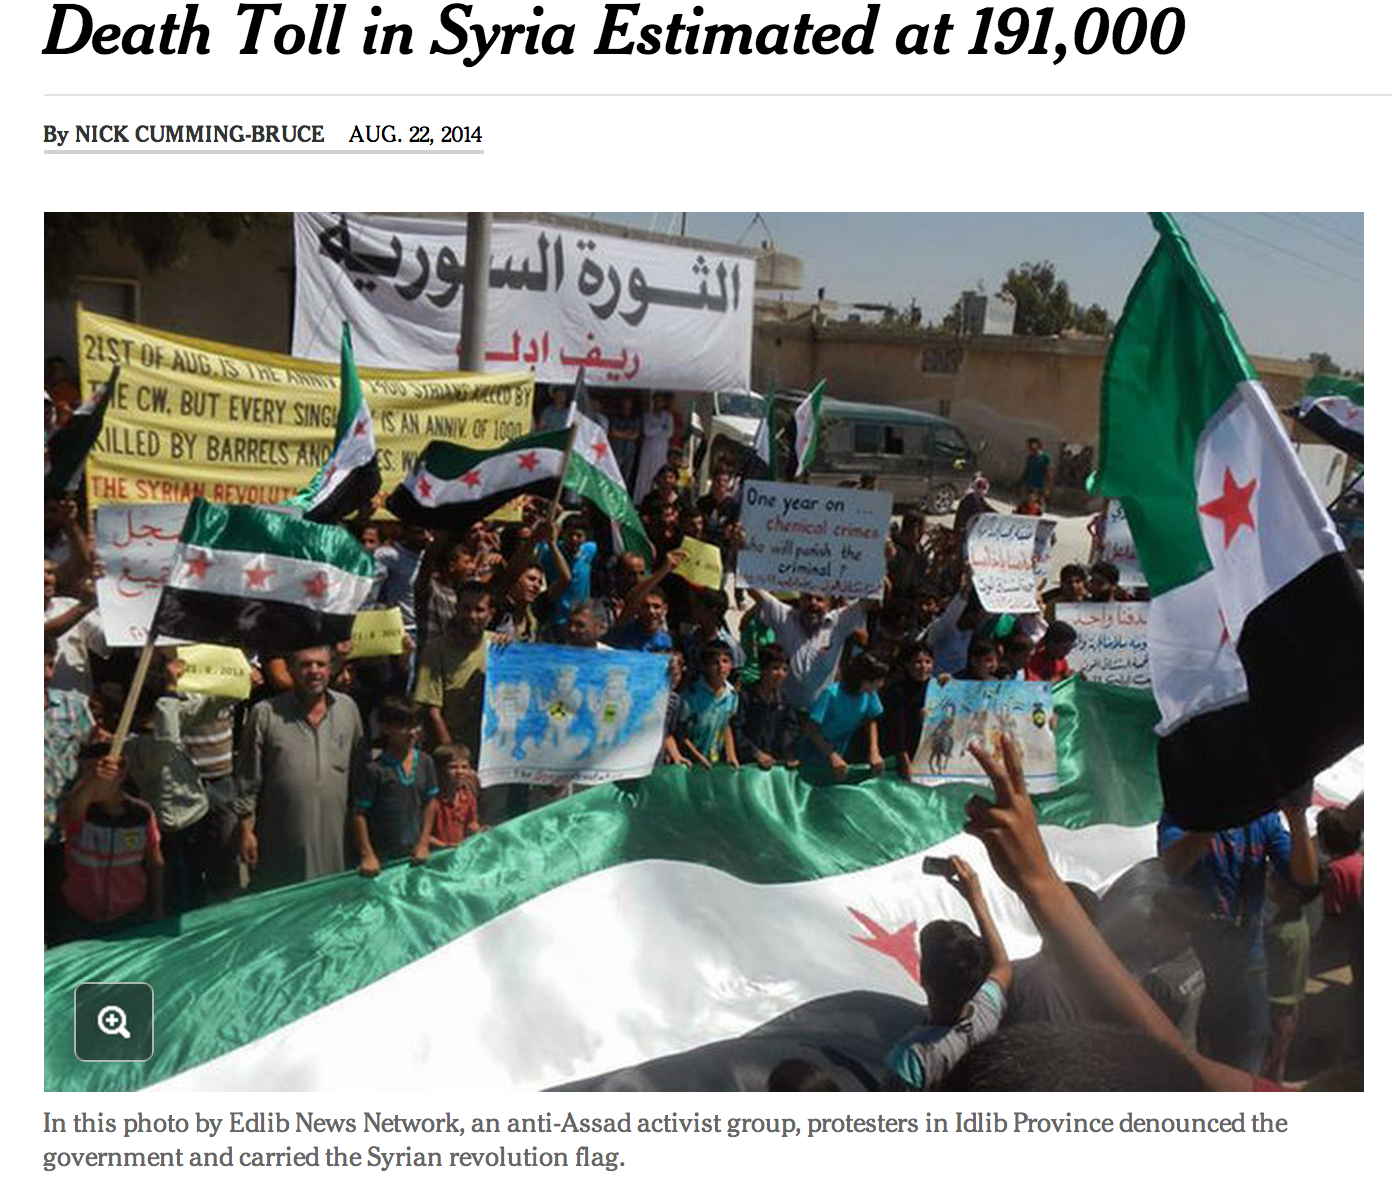
\includegraphics[width=0.7\textwidth]{figures/death_toll_aug14}
%\caption{In its third report on Syria commissioned by the United Nations, the Human Rights Data Analysis Group identified 191,369 deaths from the start of the conflict in March 2011 to April 2014, more than double the 92,901 deaths cited in the group?s last report, which covered the first two years of the conflict.}
\label{default}
\end{center}
\end{figure}

}

%\frame{
%\frametitle{Do we already know the answer?}
%
%\begin{itemize}
%\item This is a very well-documented conflict. 
%\item This is due in part to citizen journalists using:
%\begin{itemize}
%\item Twitter
%\item Facebook
%\item YouTube
%\end{itemize}
%\item Mainstream media constantly reports individuals killed in Syrian conflict.
%\end{itemize}
%
%
%}

%\frame{
%\frametitle{Data visualizations can be misleading}
%
%
%\begin{figure}[htbp]
%\begin{center}
%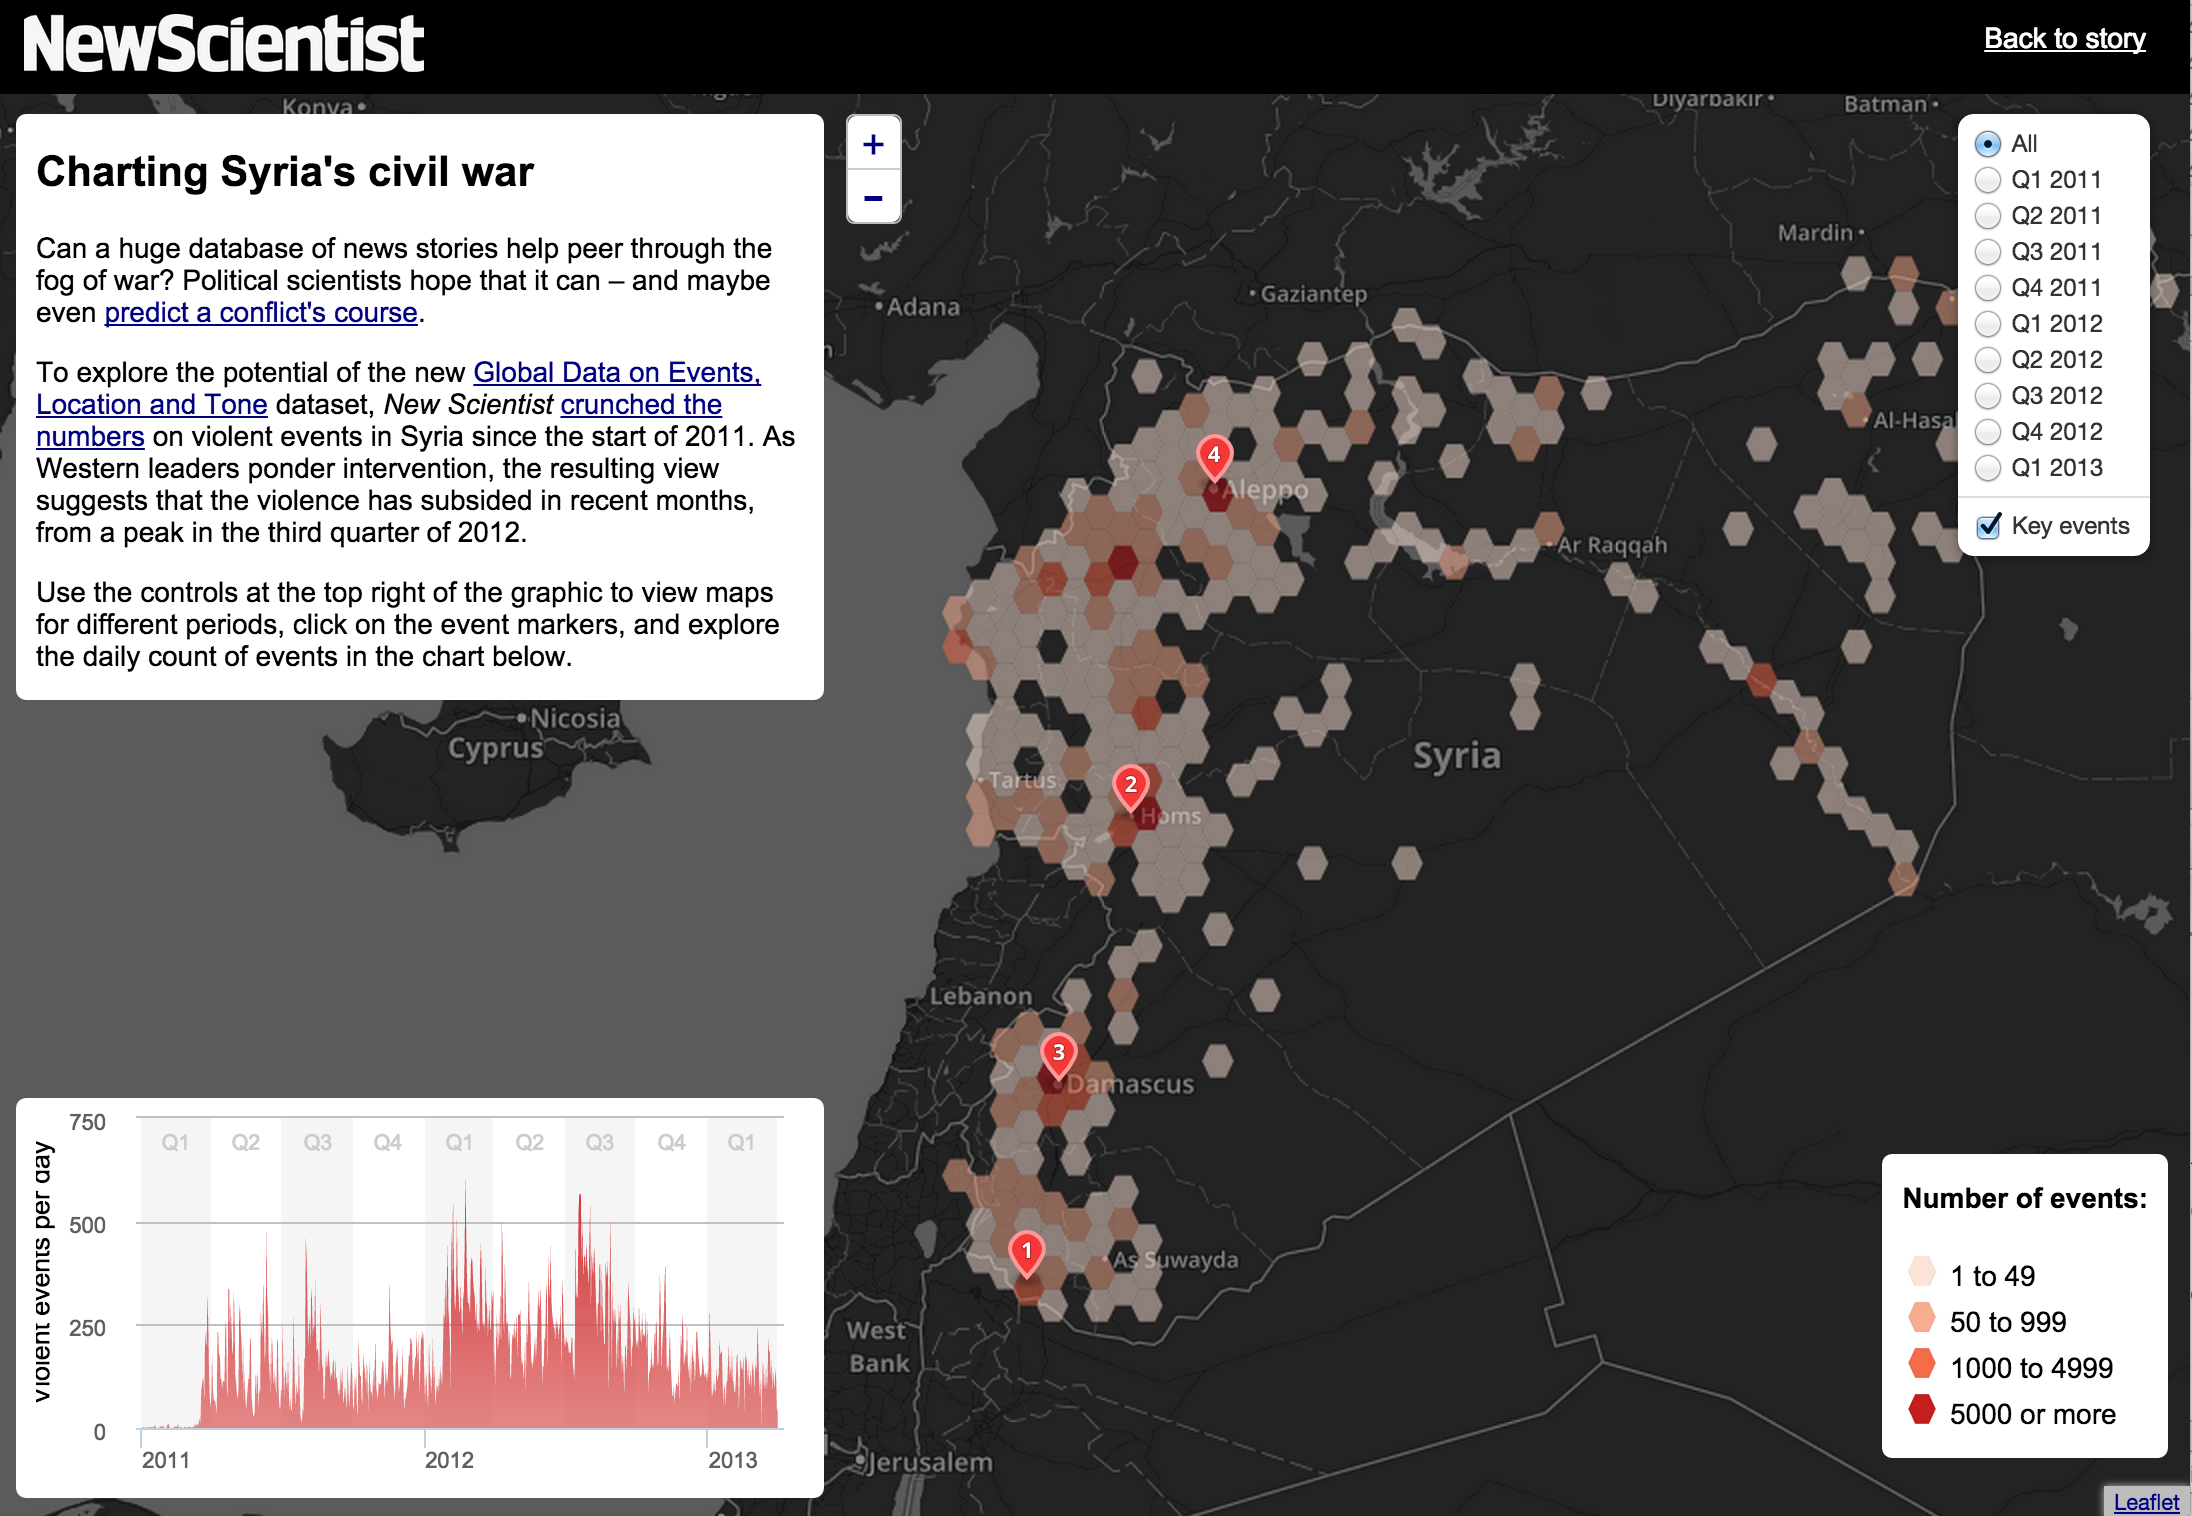
\includegraphics[width=0.8\textwidth]{figures/new_scientist}
%%\caption{default}
%\label{default}
%\end{center}
%\end{figure}
%
%}



\frame{

We build off of essential work that has been established by the Human Rights Data Analysis Group (HRDAG).


\begin{itemize}
\item We start with the raw data.
%\item Data visualizations are misleading.
%\item Natural to conclude that the violence is increasing.
%\item We have multiple data sources. 
\item We have four data sources, where the pattern over time is about the same (March 2011 --- April 2014). 
%\begin{itemize}
%\item Each source has a snapshot of different parts of the story. 
%\item However, we find by digging that the data sources are incomplete. 
%\end{itemize}
\end{itemize}

[Megan Price, Anita Gohdes, and Patrick Ball (2014)]

}



%\frame{
%\frametitle{Aleppo}
%
%\vspace*{-1em}
%\begin{figure}[htbp]
%\begin{center}
%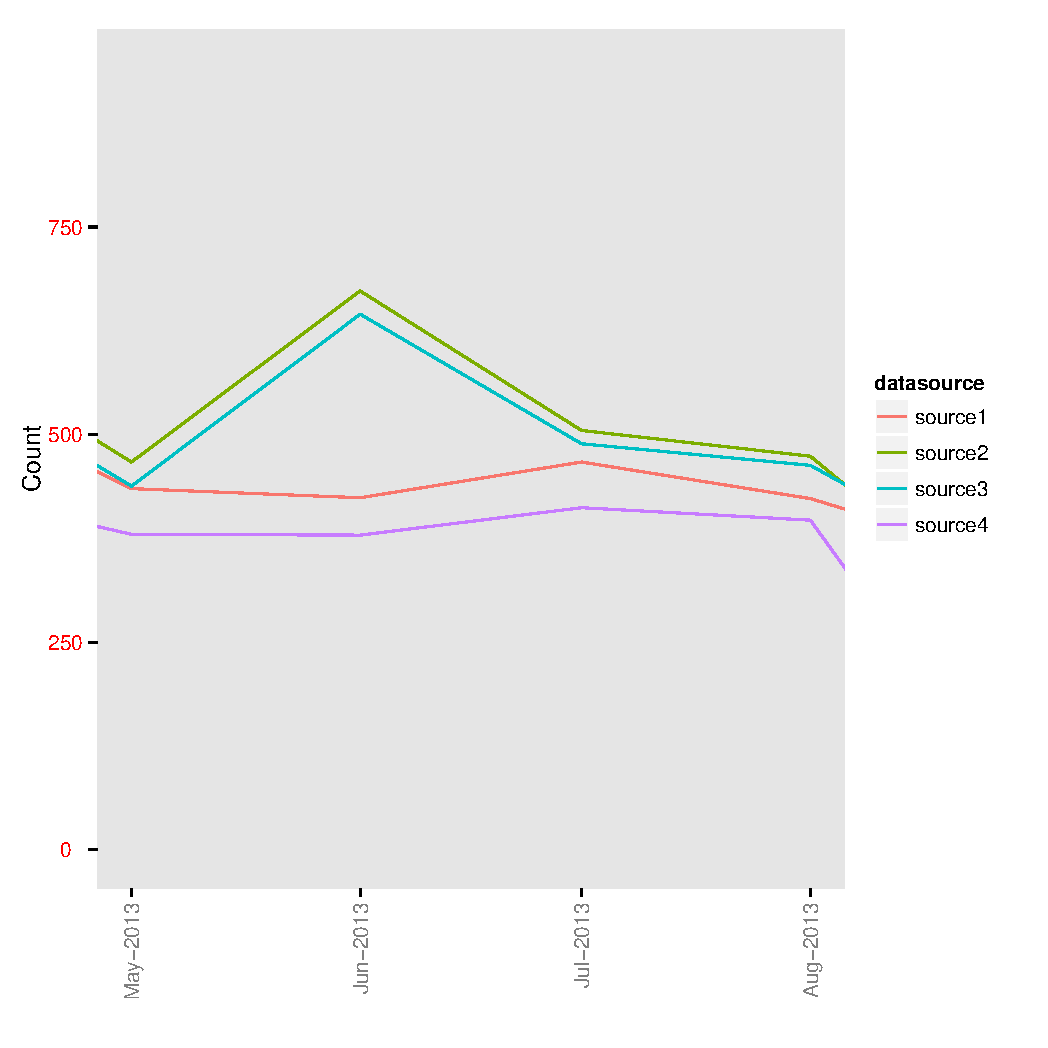
\includegraphics[width=0.7\textwidth]{figures/aleppo-2013}
%%\caption{default}
%\label{default}
%\end{center}
%\end{figure}
%
%}

%\frame{
%%\frametitle{Tartus}
%
%
%\begin{figure}[htbp]
%\begin{center}
%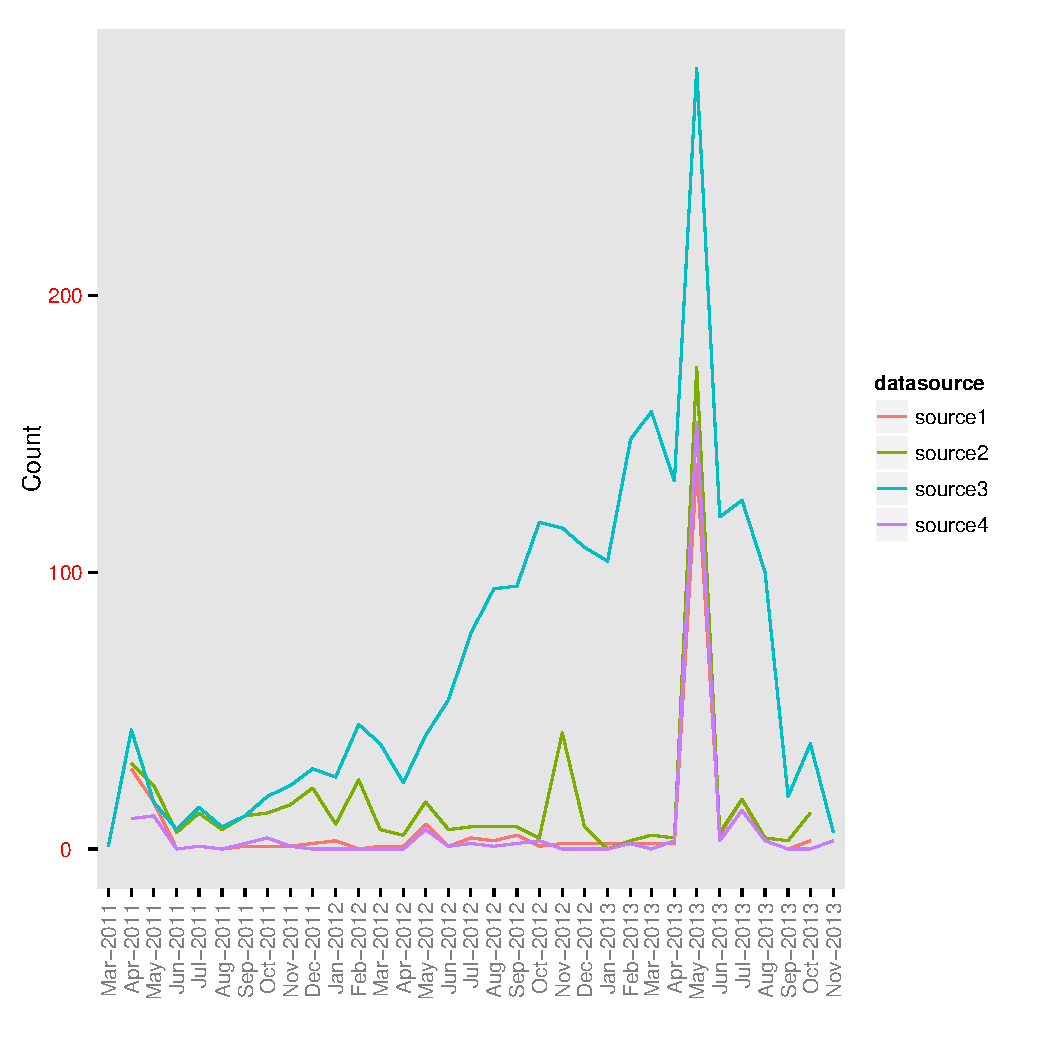
\includegraphics[width=0.7\textwidth]{figures/tartus.pdf}
%%\caption{default}
%\label{default}
%\end{center}
%\end{figure}
%
%}

%\frame{
%
%\begin{minipage}{\linewidth}
%      \centering
%      \begin{minipage}{0.45\linewidth}
%          \begin{figure}[H]
%              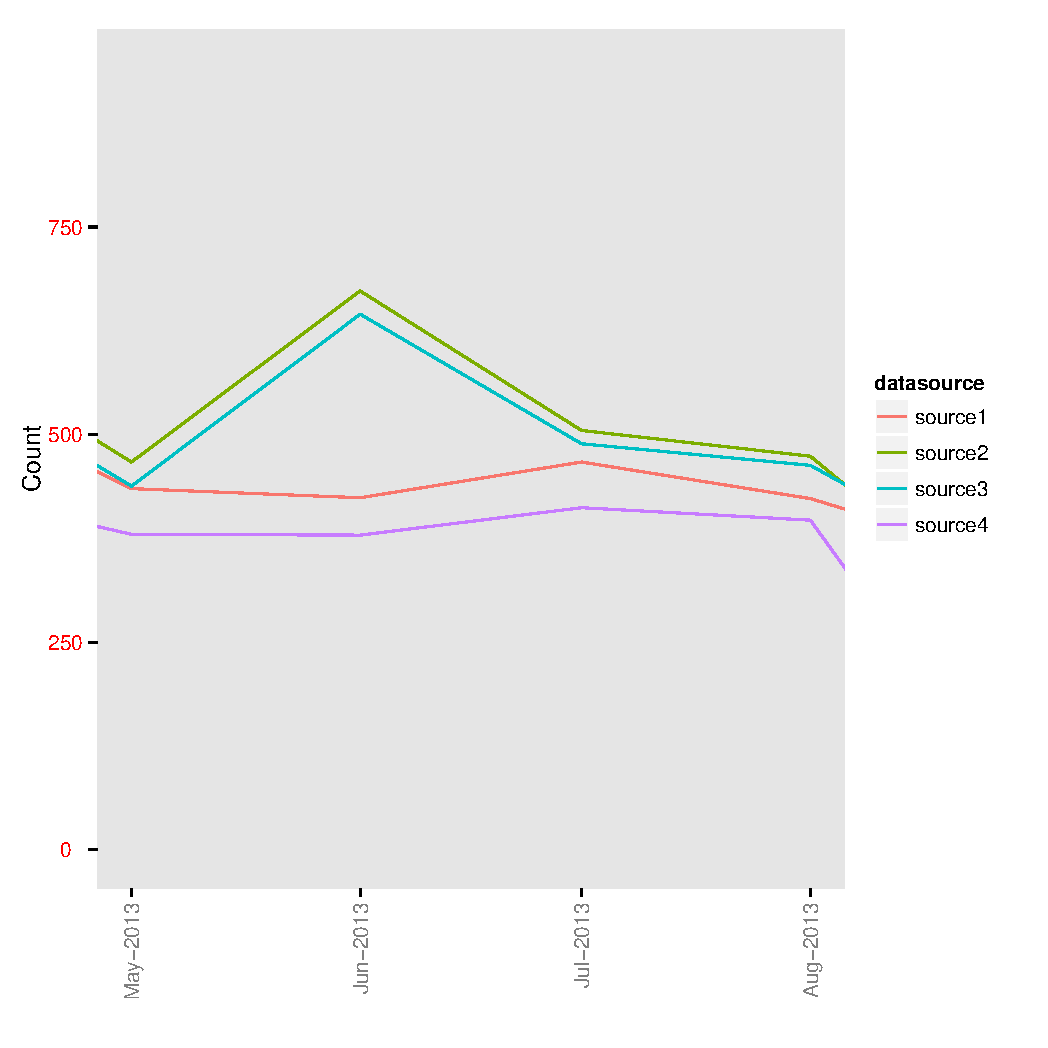
\includegraphics[width=\linewidth]{figures/aleppo-2013}
%              \caption{Aleppo, June 2013.}
%          \end{figure}
%      \end{minipage}
%      \hspace{0.05\linewidth}
%      \begin{minipage}{0.45\linewidth}
%          \begin{itemize}
%          \item Peak in violence from VDC and SNHR.
%          Violation Documentations Center (VDC) and 
%          Syrian Network for Human Rights 
%          (SNHR).
%          \item Each source has different snapshot of conflict.
%          \end{itemize}
%      \end{minipage}
%  \end{minipage}
%
%}
%
%\frame{
%
%\begin{minipage}{\linewidth}
%      \centering
%      \begin{minipage}{0.45\linewidth}
%          \begin{figure}[H]
%              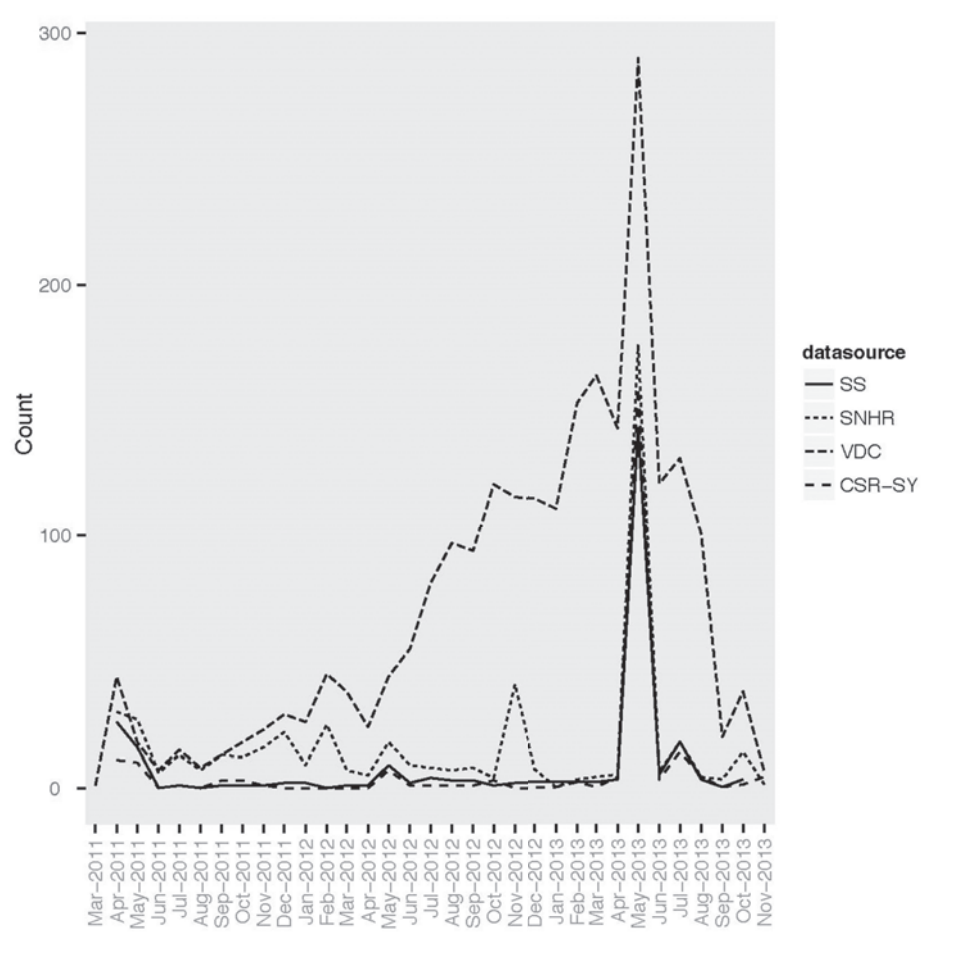
\includegraphics[width=\linewidth]{figures/tartus}
%              \caption{Leading up to massacre in Tartus, May 2013.}
%          \end{figure}
%      \end{minipage}
%      \hspace{0.05\linewidth}
%      \begin{minipage}{0.45\linewidth}
%          \begin{itemize}
%         
%\item 3 sources show this is a relatively isolated event. 
%\item VDC shows this as the culminating point of an increasing pattern of violence. 
%          \end{itemize}
%      \end{minipage}
%  \end{minipage}
%
%}



\frame{
\begin{center}
\Large
\emph{How do we attempt estimating \\ the number of  documented identifiable deaths in Syria since March 2011?}
% (in the absence of a unique identifier). 
\end{center}



}



\frame{
\frametitle{Documented, Identifiable Victims}

What resources we have:
	\begin{itemize}
	\item Human Rights Data Analysis Group collected 300,000 death records from Syria, which was published in a 2014 report with the United Nations.
\item Records reported from four human rights sources. 
\item Field attributes: Full Arabic name, date of death (DOD), governorate, other less reliable ones. 
		\item 40,000 record pairs labeled as match/non-match.
%		\item 200,000+ record pairs labeled as match/non-match\\(coming soon, hopefully) 
	\end{itemize}


}





%\frame{
%
%
%\begin{figure}[htbp]
%\begin{center}
%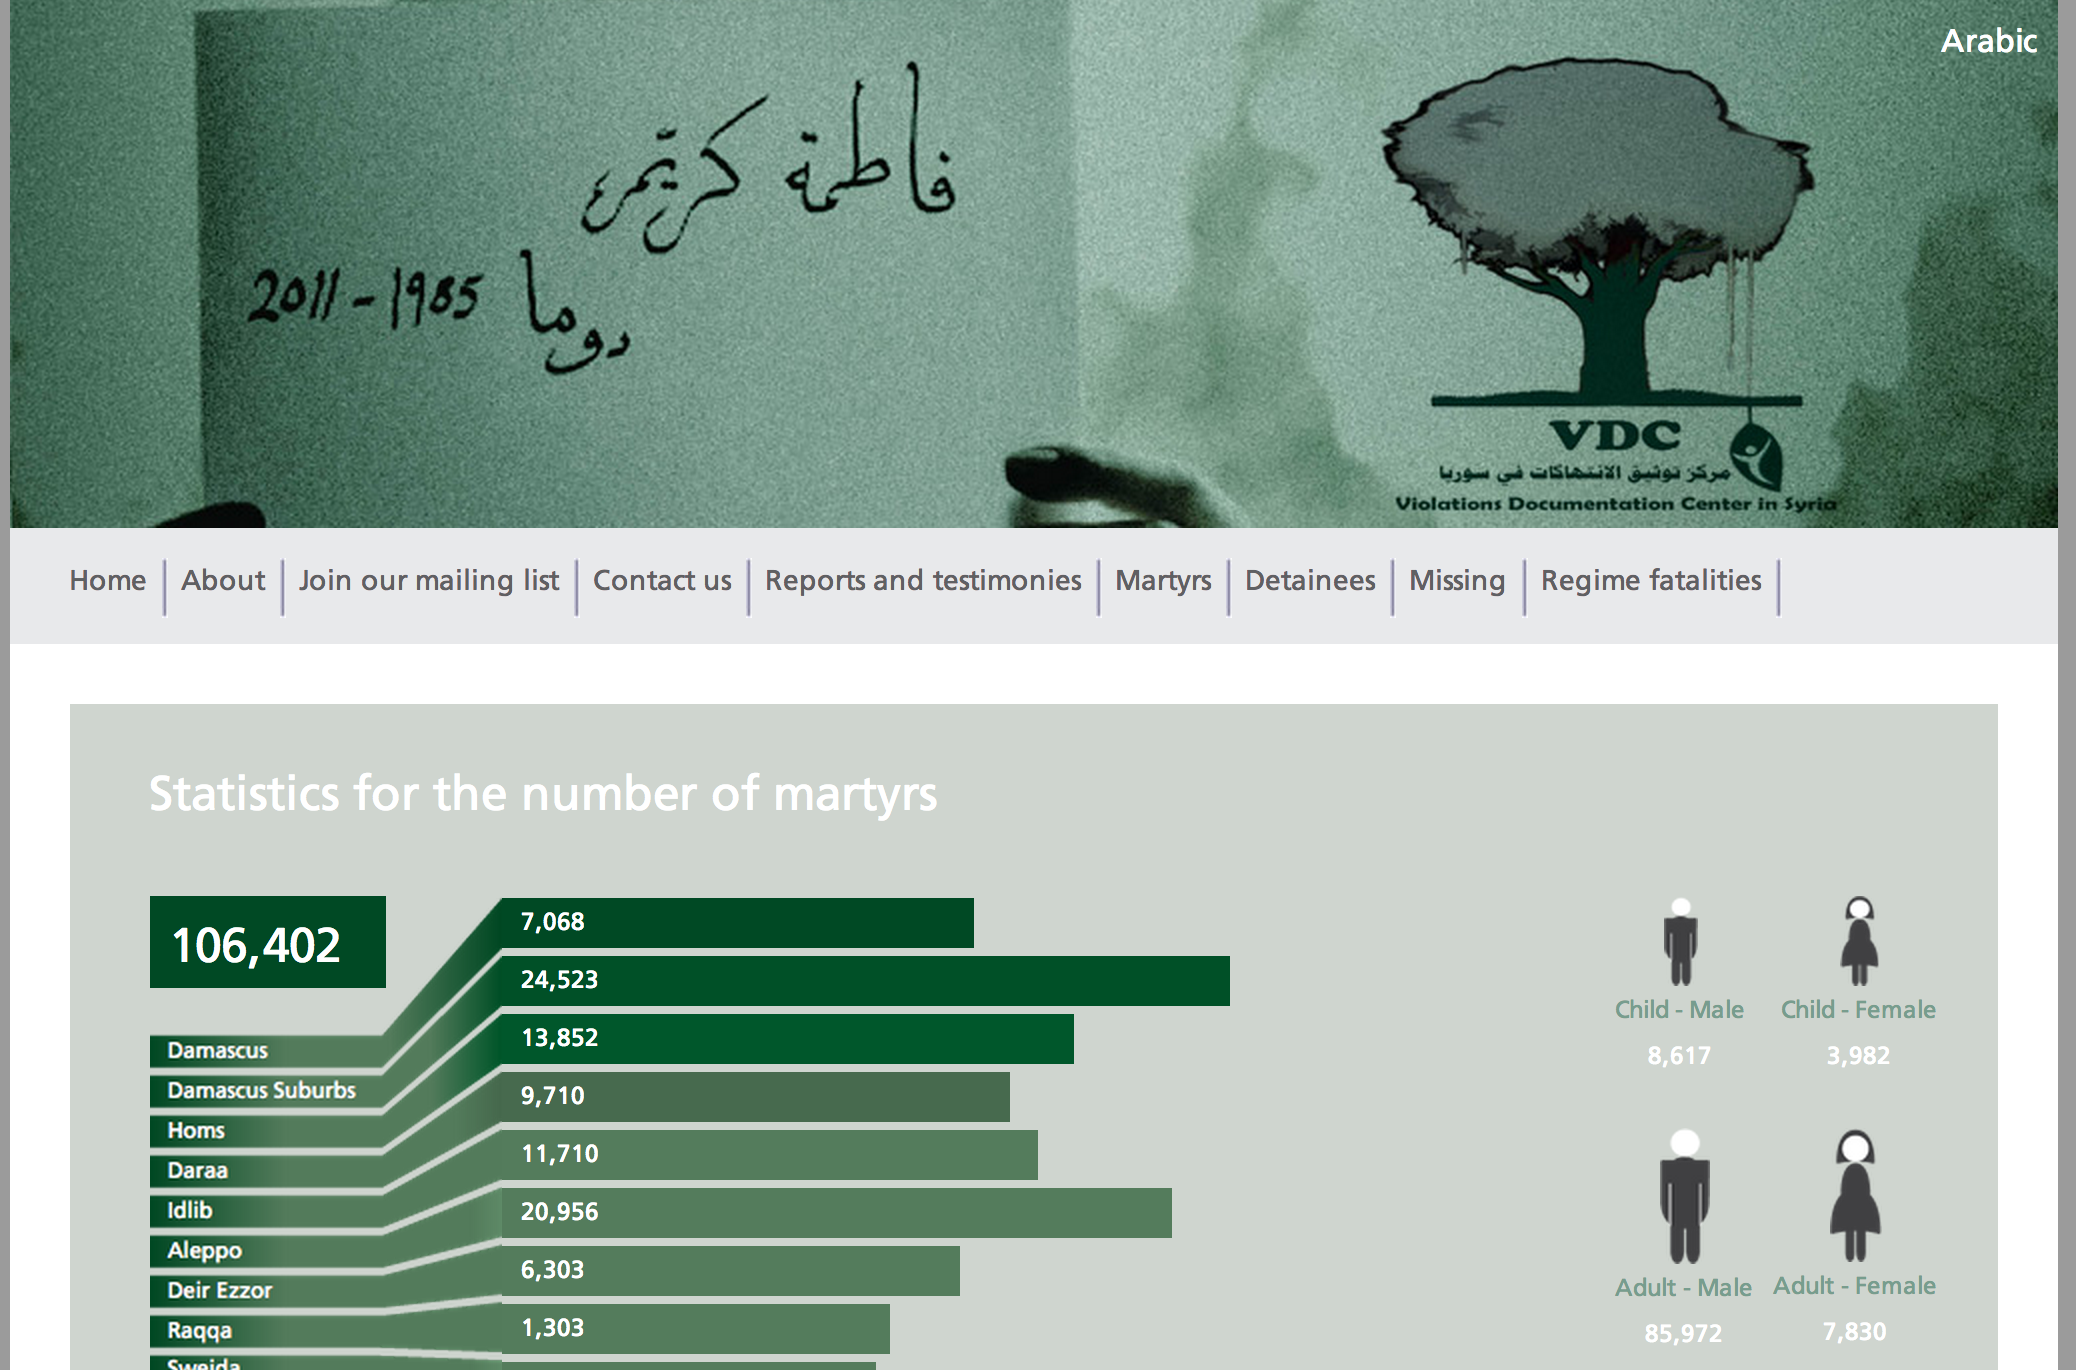
\includegraphics[width=\textwidth]{figures/vdc}
%%\caption{default}
%\label{default}
%\end{center}
%\end{figure}
%
%}


\frame{
\frametitle{HRDAG's August 2014 Release}

\begin{itemize}
\item Estimated 191,000 documented, identifiable deaths. 
\item Used hand matching (five people). 
\end{itemize}

\begin{enumerate}
\item How reliable is the hand matching? 
\item Standard error.
\item Scalability and cost. 
\end{enumerate}

How can we improve on this approach?


}



\frame{

\begin{center}
\Large
\emph{Entity resolution (record linkage or de-duplication) joins multiple data sets removes duplicate entities often in the absence of a unique identifier.}
% (in the absence of a unique identifier). 
\end{center}

%%\vspace*{-1.5em}
%\begin{figure}[htbp]
%\begin{center}
%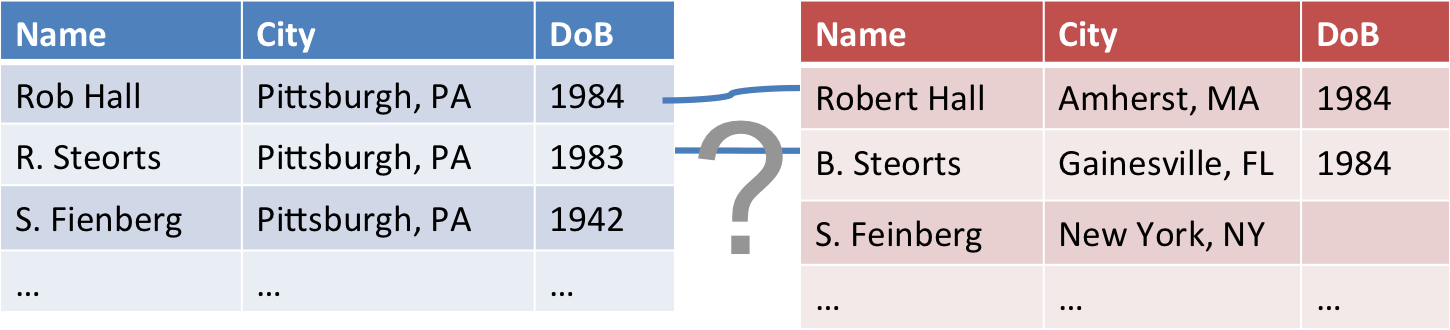
\includegraphics[scale=0.45]{figures/link_names.png}
%%\caption{default}
%%\label{default}
%\end{center}
%\end{figure}
%
%The linkage between individuals can also be represented as edges in a graph (the records are nodes). 



}

\frame{
\frametitle{The record linkage graph}
\begin{figure}[htbp]
\begin{center}
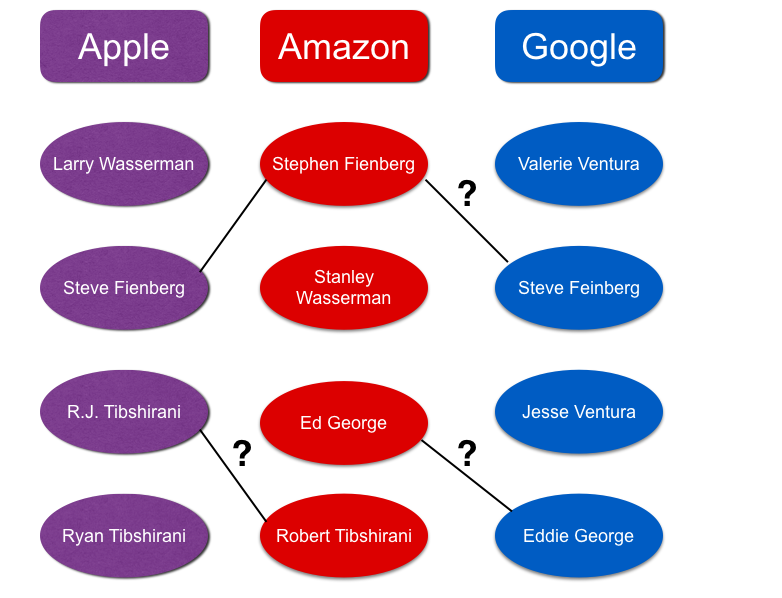
\includegraphics[scale=0.35]{figures/linkage2}
%\caption{default}
%\label{default}
\end{center}
\end{figure}

}


%\subsection{Application to Syrian War}
\frame{
\frametitle{The Syrian record linkage graph}
\vspace*{-0.75em}
\begin{figure}[htbp]
\begin{center}
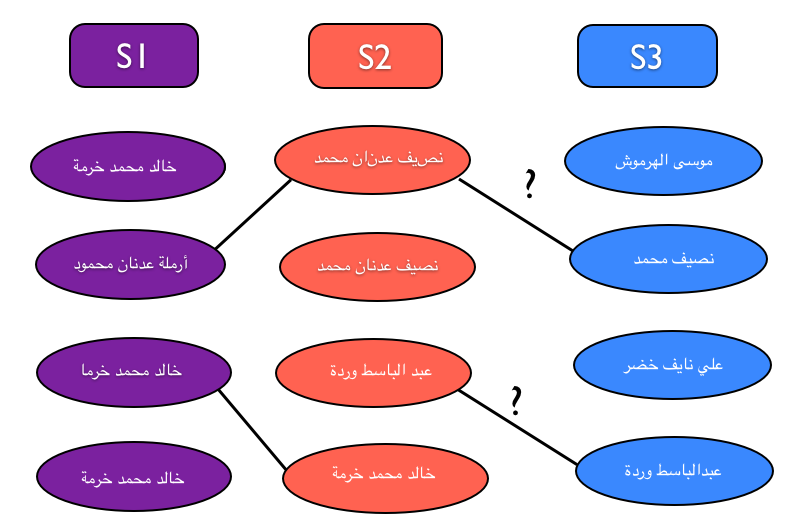
\includegraphics[scale=0.35]{figures/syrian}
%\caption{default}
%\label{default}
\end{center}
\end{figure}

%\begin{flushright}
%Steorts (2014, To be Submitted, AIStats)
%\end{flushright}



}





%\frame{
%\begin{figure}[htbp]
%\vspace*{-1em}
%\begin{center}
%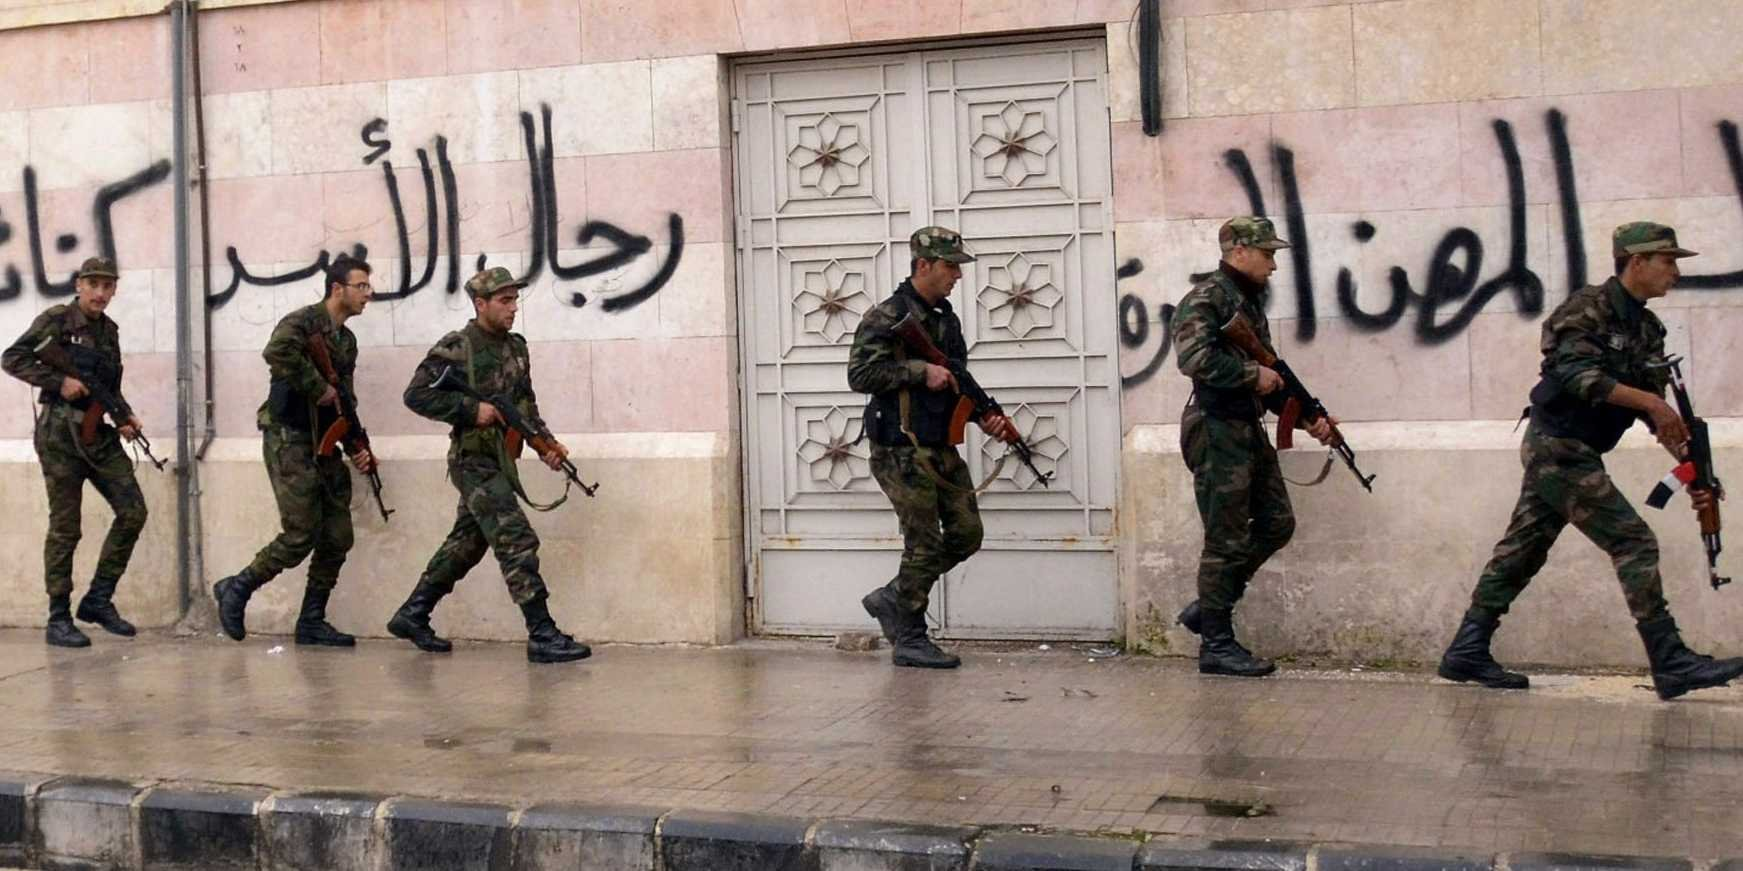
\includegraphics[scale=0.18]{figures/asad.jpg}
%%\caption{default}
%\end{center}
%\small
%``The `complex and dangerous' nature of Syria's civil war has made it impossible to accurately update the death toll that last stood at around 100,000 people."\\
%%\vspace*{1em}
%---spokesman from the United Nations on Jan.\ 7, 2014
%\end{figure}
%}
%
%
%\frame{
%
%
%\begin{figure}[htbp]
%\vspace*{-1em}
%\begin{center}
%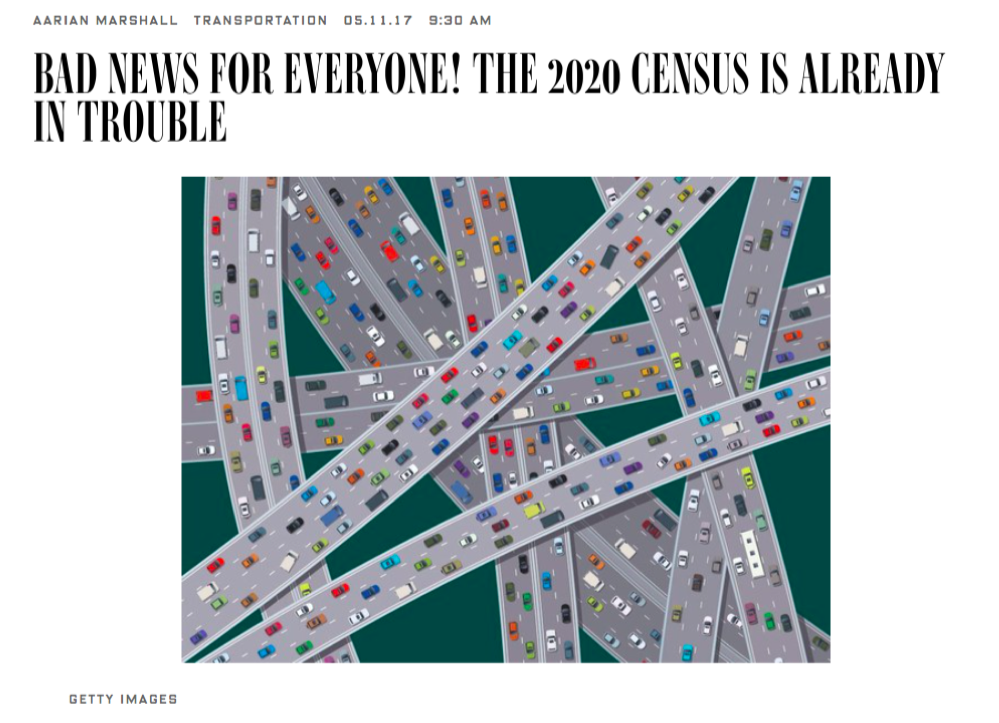
\includegraphics[scale=0.3]{figures/census2}
%%\caption{default}
%\end{center}
%\end{figure}
%
%
%}


%
%\frame{
%\begin{figure}[htbp]
%\begin{center}
%\includegraphics[scale=0.35]{pics_sm/google_jsm.pdf}
%%\caption{default}
%%\label{default}
%\end{center}
%\end{figure}
%
%
%
%}
%
%\frame{
%\begin{figure}[ht]
%\begin{minipage}[b]{0.45\linewidth}
%\centering
%
\includegraphics[width=\textwidth]{figures/steve_1}
%%\caption{default}
%%\label{fig:figure1}
%\end{minipage}
%\hspace{0.5cm}
%\begin{minipage}[b]{0.45\linewidth}
%\centering
%
\includegraphics[width=\textwidth]{figures/blank}
%%\caption{default}
%%\label{fig:figure2}
%\end{minipage}
%\end{figure}
%}
%
%\frame{
%\begin{figure}[ht]
%\begin{minipage}[b]{0.45\linewidth}
%\centering
%
\includegraphics[width=\textwidth]{figures/steve_1}
%%\caption{default}
%%\label{fig:figure1}
%\end{minipage}
%\hspace{0.5cm}
%\begin{minipage}[b]{0.45\linewidth}
%\centering
%
\includegraphics[width=\textwidth]{figures/steve_2}
%%\caption{default}
%%\label{fig:figure2}
%\end{minipage}
%\end{figure}
%\pause
%
%These are clearly not the \emph{same} Steve Fienberg!
%
%
%}
%
%%\subsection{Application to Syrian War}
%\frame{
%\frametitle{Syrian Civil War}
%\vspace*{-0.75em}
%\begin{figure}[htbp]
%\begin{center}
%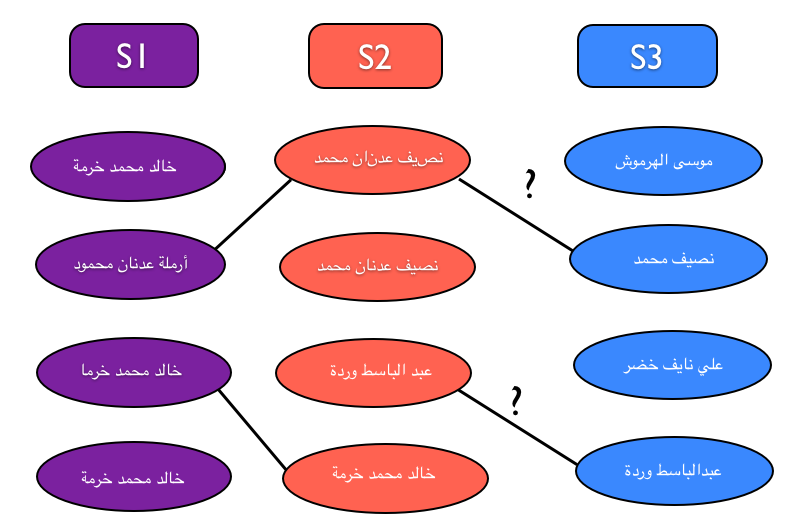
\includegraphics[scale=0.35]{figures/syrian}
%%\caption{default}
%%\label{default}
%\end{center}
%\end{figure}
%
%%\begin{flushright}
%%Steorts (2014, To be Submitted, AIStats)
%%\end{flushright}
%
%
%
%}





\frame{
\frametitle{Entity Resolution}
\Large
%\emph{Now, we can run any record linkage procedure in parallel once the blocks
%are created. How to do this?}\\

%\vspace*{1em}
\center
\emph{Why is entity resolution difficult?}

}


%\frame{
%\frametitle{Goals of Entity Resolution}
%
%%\emph{Now, we can run any record linkage procedure in parallel once the blocks
%%are created. How to do this?}\\
%
%%\vspace*{1em}
%
%Suppose that we have a total of $M$ records in $D$ data sets. 
%
%\begin{enumerate}
%\item We seek models that are much less than $O(M^2)$ (quadratic).
%\item We seek models that are reliable, accurate, fit the data well, and account for the uncertainty of the model.
%\end{enumerate}
%
%\pause
%These two goals fundamentally go against one another, making record linkage a very challenging problem.
%\vspace*{1em}
%\pause
%
%%In this talk, we will focus on (2) since satisfying the above goals is very difficult. 
%
%%Depending on the motivating goal of a record linkage task, we approach it using either 1 or 2. 
%
%}

%\frame{
%
%Suppose that we have a total of $M$ records in $D$ data sets. 
%
%\begin{enumerate}
%\item We seek models that are much less than $O(M^2)$ (quadratic).
%\item We seek models that are reliable, accurate, fit the data well, and account for the uncertainty of the model.
%\end{enumerate}
%
%In the rest of the talk, we will
%\begin{enumerate}
%\item Review the literature.
%\item Present Bayesian methods that satisfy 2.
%\item And present a framework that satisfies both 1 and 2 (with a restriction). 
%\end{enumerate}
%
%}
%
%
%\frame{
%\frametitle{Common Methods for Entity Resolution}
%
%
%\begin{itemize}
%\item Match on a unique identifier if it exists.
%\item Perform exact matching.
%\item Perform a likelihood ratio or hypothesis test. 
%\end{itemize}
%
%[Newcombe (1959), Fellegi and Sunter (1969)]. 
%
%}
%
%\begin{frame}
%\frametitle{My Frustrations, Let Me Show You Them}
%Assume $M$ total records.
%\begin{itemize}
%\item Needs $O(M^2)$ record comparisons.
%\item No natural way of quantifying uncertainty of the entity resolution process under the ``common methods".
%\item Awkward to extend to more than $k=2$ files:
%\begin{itemize}
%\item Hypothesis tests on triples (quadruples, $k$-tuples) of records with multiple alternative hypotheses.
%\item Or just do pairwise linkage, and try to reconcile the different file pairs somehow.
%\end{itemize}
%%\item Duplicate files must be handled.
%%\item Lack of transitivity of records is an issue.
%%\begin{itemize}
%%\item De-duplication and transitivity resolved in \cite{sadinle_multi_1}.
%%\item Computationally infeasible for moderate $k.$
%%\end{itemize}
%\end{itemize}
%
%This problem is just messy and difficult! 
%\end{frame}
%
%\frame{
%\frametitle{Bayesian graphical entity resolution}
%
%We review recent Bayesian methods that 
%are reliable, accurate, fit the data well, and account for the uncertainty of the entity resolution process. 
%
%\vspace*{2em}
%
%In addition, a large class of these methods have sound theoretical properties. 
%
%}
%
%\frame{
%\frametitle{Recent Bayesian methods}
%
%\begin{itemize}
%\pause
%\item Dealing with big data means merging large, noisy databases.
%\pause
%\begin{itemize}
%\item Such databases have severe amounts of noise. 
%\end{itemize}
%\pause
%\item Entity resolution requires sophisticated graph structures. [Gutman et. al (2013)].
%\pause
%\begin{itemize}
%\item One approach is to use a bipartite graph for latent entities.
%\pause
%\item Never link records to records. 
%\pause
%\end{itemize}
%\item Computational speed-ups: eliminate low-probability matches.
%%\pause
%%\begin{itemize}
%%\item Blocking techniques based on locality-sensitive hashing.
%\end{itemize}
%\pause
%
%\begin{figure}[htbp]
%\begin{center}
%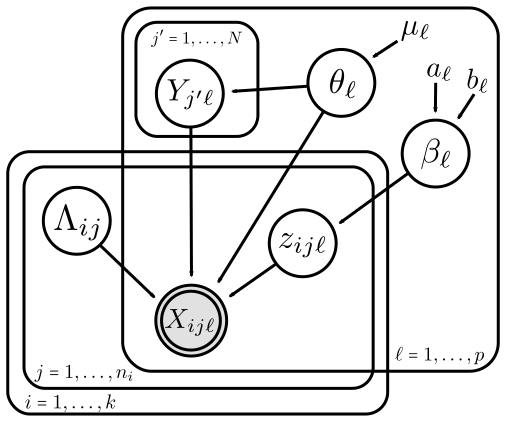
\includegraphics[width=0.35\textwidth]{figures/recordLinkage_graphicalModel}
%%\caption{Graphical representation of models \ref{model:cat}-\ref{model:string}.}
%\label{fig:graphicalProcess}
%\end{center}
%\end{figure}
%
%
%[Tancredi and Liseo (2011), \textbf{RCS}, Hall, Fienberg (2014, 2016); Sadinle (2014, 2016); 
%\textbf{RCS} (2015)]. 
%
%
%}
%
%\frame{
%
%\begin{figure}[htbp]
%\begin{center}
%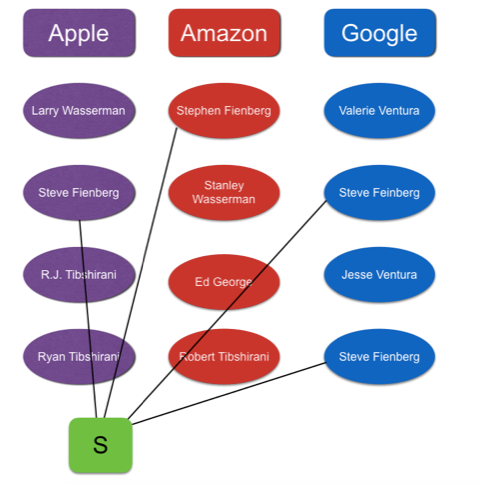
\includegraphics[scale=0.35]{figures/latent1}
%%\caption{default}
%%\label{default}
%\end{center}
%%\scriptsize{
%%\begin{flushright}
%%[Steorts, Hall, and Fienberg (2014), \emph{AIStats}.] \newline
%%[Steorts, Hall, and Fienberg (2014), \emph{JASA}, In Revision.], [Steorts (2014), Submitted.] 
%%\end{flushright}
%%}
%\end{figure}
%
%}
%
%
%\frame{
%
%\begin{figure}[htbp]
%\begin{center}
%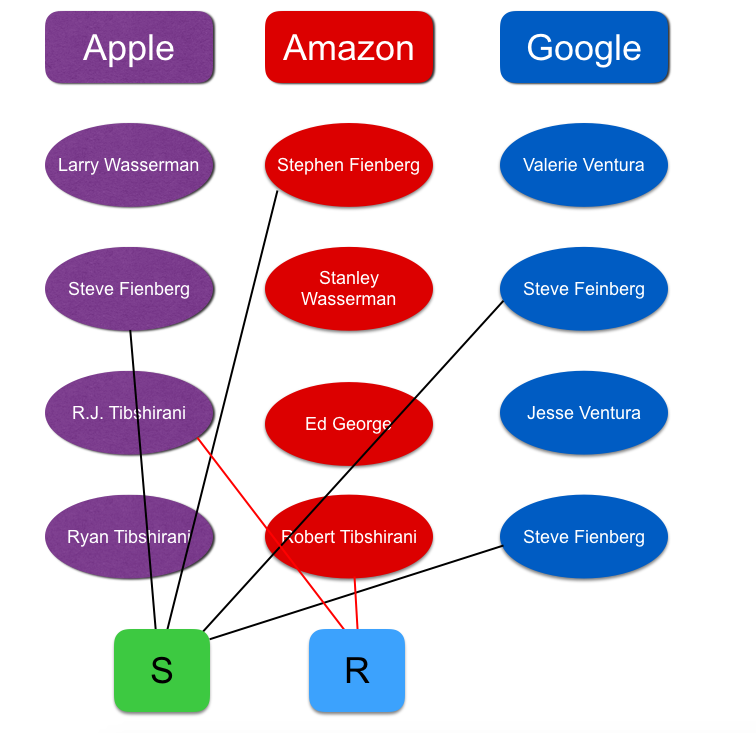
\includegraphics[scale=0.35]{figures/latent2}
%%\caption{default}
%%\label{default}
%\end{center}
%%\scriptsize{
%%\begin{flushright}
%%[Steorts, Hall, and Fienberg (2014), \emph{AIStats}.] \newline
%%[Steorts, Hall, and Fienberg (2014), \emph{JASA}, In Revision], [Steorts (2014), Submitted.] 
%%\end{flushright}
%%}
%\end{figure}
%
%}
%
%
%%\frame{
%%
%%\begin{figure}[htbp]
%%\begin{center}
%%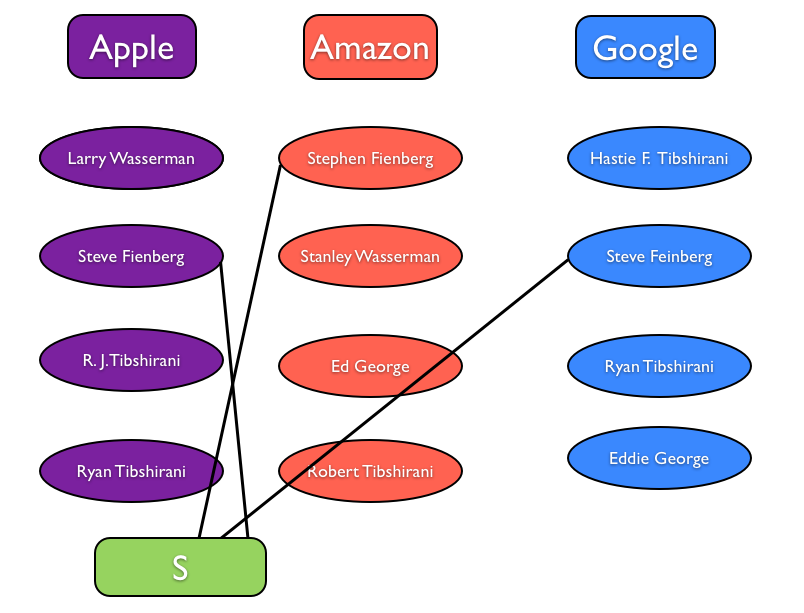
\includegraphics[scale=0.35]{figures/latents_firstex}
%%%\caption{default}
%%%\label{default}
%%\end{center}
%%%\scriptsize{
%%%\begin{flushright}
%%%[Steorts, Hall, and Fienberg (2014), \emph{AIStats}.] \newline
%%%[Steorts, Hall, and Fienberg (2014), \emph{JASA}, In Revision.], [Steorts (2014), Submitted.] 
%%%\end{flushright}
%%%}
%%\end{figure}
%%
%%}
%%
%%
%%\frame{
%%
%%\begin{figure}[htbp]
%%\begin{center}
%%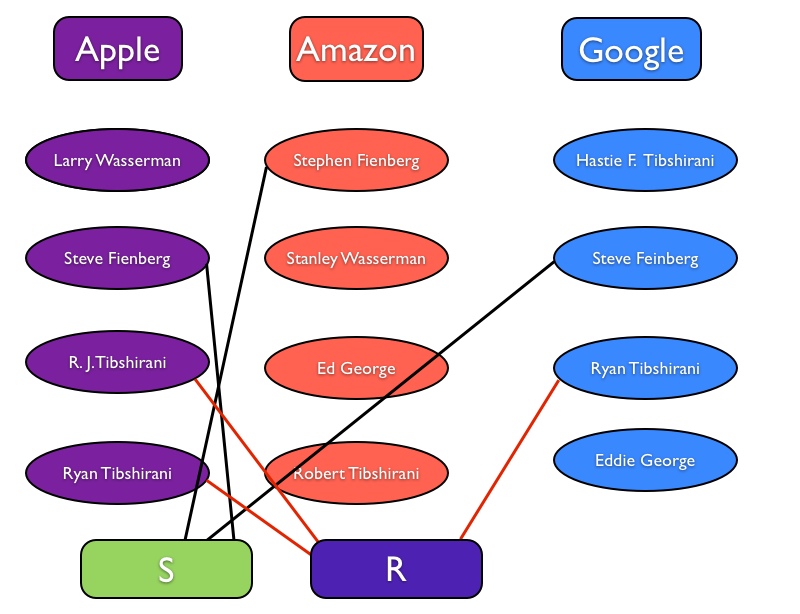
\includegraphics[scale=0.35]{figures/latents_secondex}
%%%\caption{default}
%%%\label{default}
%%\end{center}
%%%\scriptsize{
%%%\begin{flushright}
%%%[Steorts, Hall, and Fienberg (2014), \emph{AIStats}.] \newline
%%%[Steorts, Hall, and Fienberg (2014), \emph{JASA}, In Revision], [Steorts (2014), Submitted.] 
%%%\end{flushright}
%%%}
%%\end{figure}
%%
%%}
%
%\frame{
%\frametitle{Extension to Text Data}
%%Previous literature: not balanced regarding modeling and handling high-dimensional data.
%\vspace*{1em}
%%Propose a parametric Bayesian 
%%model that simultaneously links records and de-duplicates. 
%\begin{itemize}
%\item  Extension of \textbf{RCS}, Hall, Fienberg (2014, 2016) to both categorical and text data, on real data sets with comparisons to many different methods. 
%\item Takes an empirical Bayes approach.
%\item Comparisons to supervised methods, beating them!
%\end{itemize}
%
%
%[\textbf{RCS} (2015), \emph{Bayesian Analysis}, Finalist for Lindley Prize.] \\
%\href{https://cran.r-project.org/web/packages/blink/index.html}{\texttt{R} package \texttt{blink} on CRAN and github}
%
%}
%
%
%
%\frame{
%\frametitle{EB Approach}
%
%\begin{itemize}
%%\item Clusters records to latent individuals using an EB approach. 
%%\item Incorporates both categorical and string data.
%%\item The probability of observing a given word is $\propto$ the empirical frequency of the word times $c.$
%% \item $c$ shrinks exponentially in the distance from the true value.
%\item When a string-valued field in a record is distorted from the true latent value, the distorted value is distributed as
%\[
%\Pr(\text{observe string }w^{\prime} \mid \text{true string }w) \propto \Pr_{\text{empirical}}(w^{\prime})\;e^{-c\,d(w^{\prime},w)}.
%\] 
%%\item The string metric $d$ is general and decided by the user. % Can be validated using traditional methods.
%%\item All the full conditionals are in closed form. 
%\end{itemize}
%\begin{flushright}
%[\textbf{RCS} (2015), \emph{Bayesian Analysis}, Finalist for Lindley Prize.]
%\end{flushright}
%
%}
%
%\frame{
%\frametitle{Empirical Bayes Model }
%\small
%\begin{itemize}
%\item Define
%$
%\alpha_\ell(w)=
%%\frac{1}{N}\sum_{i=1}^k\sum_{j=1}^{n_i}I(X_{ij\ell}=w).%=
%\text{relative frequency of $w$ in data for field $\ell$}.
%$
%\pause
%\item $G_\ell$: empirical distribution for field $\ell.$
%%\item $W \sim G_\ell, \implies \forall w$,
%%$
%%P(W=w)=\alpha_\ell(w).
%%$
%\pause
%\item $W\sim F_\ell(w_0)$: $\textcolor{black}{P(W=w)\propto\alpha_\ell(w)\,\exp\!\left[-c\,d(w,w_0)\right],}$
%where $d(\cdot,\cdot)$ is a string metric and $c>0$.
%\end{itemize}
%\pause
%\vspace*{-1em}
%\begin{align*}
%X_{ij\ell}\mid \lambda_{ij},\,Y_{\lambda_{ij}\ell},\,z_{ij\ell}\;&\sim\begin{cases}\delta(Y_{\lambda_{ij}\ell})&\text{ if }z_{ij\ell}=0\\F_\ell(Y_{\lambda_{ij}\ell})&\text{ if }z_{ij\ell}=1\text{ and field }\ell\text{ is string-valued}\\G_\ell&\text{ if }z_{ij\ell}=1\text{ and field }\ell\text{ is categorical}\end{cases}\\
%%&\qquad\text{for each }i\in\{1,\ldots,k\},\; j\in\{1,\ldots,n_i\},\; \ell\in\{1,\ldots,p_s+p_c\},\\
%%&\qquad\text{with everything independent},\\
%Y_{j'\ell}\;&\sim G_\ell\\
%z_{ij\ell}\mid\beta_{i\ell}\;&\sim \text{Bernoulli}(\beta_{i\ell})\\
%\beta_{i\ell}\;&\sim\text{Beta}(a,b)\\
%\lambda_{ij}\;&\sim\text{DiscreteUniform}(1,\ldots,N_{\max}),\quad
%\text{ where }N_{\max}=\sum_{i=1}^k n_i.
%\end{align*}
%%with everything independent of everything else.
%
%
%}
%
%\frame{
%\frametitle{Microclustering}
%
%The above work led to discovery that many clustering algorithms for Bayesian non-parametrics are inappropriate for entity resolution. 
%\pause
%
%\vspace*{1em}
%
%The cluster sizes grow sub-linearly with the number of records.
%
%\pause
%\vskip 1em
%A sequence of random partitions $(C_N
%: N=1, 2, \ldots)$ exhibits the \emph{microclustering property} if $M_N$ is
%$o_p(N)$, where $M_N$ is the size of the largest cluster in
%$C_N$. 
%%Equivalently, $M_N \,/\, N \rightarrow 0$ in probability as $N
%%\rightarrow \infty$.
%
%\pause
%\vskip 1em
%A clustering model exhibits the microclustering property if $(C_N
%: N=1, 2, \ldots)$  implied by that model satisfies the above definition.
%
%\vskip 1em
%
%
%[Zanella, Betancourt, Wallach, Miller, Zaidi, and \textbf{RCS} (2016)]\\
%NSF CAREER Award 2017
%}
%
%\frame{
%\frametitle{Theoretical Limits for  Entity Resolution}
%Are there theoretical limits for entity resolution? Yes! 
%
%\vspace*{1em}
%
%Two very different approaches:
%
%\begin{enumerate}
%\item Johndrow, Lum, and Dunson, Under Review, 2017.
%\begin{itemize}
%\item The authors show that that for $p$ features or when the number of entities is small compared to the number of records that entity resolution is ``effectively impossible." 
%\end{itemize}
%\item \textbf{RCS}, Barnes, Neiswanger (2017), AIStats, \url{http://proceedings.mlr.press/v54/}.
%\begin{itemize}
%\item We derive performance bounds using the KL divergence on when a latent entity is mis-classified, showing when the bounds are tight.
%\end{itemize}
%\end{enumerate} 
%
%\begin{itemize}
%\item The first paper sheds light on the implausibility of entity resolution. The second paper sheds light on the plausibility and implausibility of entity resolution. 
%
%\item By combining approaches in both papers, we may find further insights on both theoretical and practical entity resolution. 
%\end{itemize}
%}
%
%
%\frame{
%\frametitle{Performance Bounds for Graphical Entity Resolution}
%%Recall the connection to KL divergence in the sense that for any two distributions $P$ and $Q$, the maximum power for testing $P$ versus $Q$ is $\exp\{-n D_{\text{KL}}(P || Q)\}.$ 
%%
%%\vspace*{1em}
%%Hence, a low value of $D_{KL}$ means that we need many samples to distinguish $P$ from $Q.$ 
%
%There are two natural questions that can be addressed from \textbf{RCS}, Barnes, Neiswanger (2017), AIStats.
%
%\begin{enumerate}
%\item How  does changing $\textbf{Y}$ (latent entity) or $\lam$ (linkage structure) change the distribution of $\bX$ (observed records)? 
%%We search for both meaningful upper and lower bounds, since an upper bound will say that $P$ and $Q$ are never more than so far apart, whereas a lower bound says how easy it is to tell $P$ and $Q$ apart. 
%\item Moreover, we investigate how well can we recover $\bY$ (latent entity) and $\lam$ (linkage structure) from $\bX$ (data).
%\end{enumerate}
%
%}
%
%\frame{
%\frametitle{Performance Bounds for Graphical Entity Resolution }
%
%
%
%%\begin{itemize}
%%\item T
%%%\item For simulation results, gives guidance for when the bounds are loose and when they are tight, which matches 
%%%the previous literature on partition models.
%%\end{itemize}
%
%\begin{figure}[htbp]
%\begin{center}
%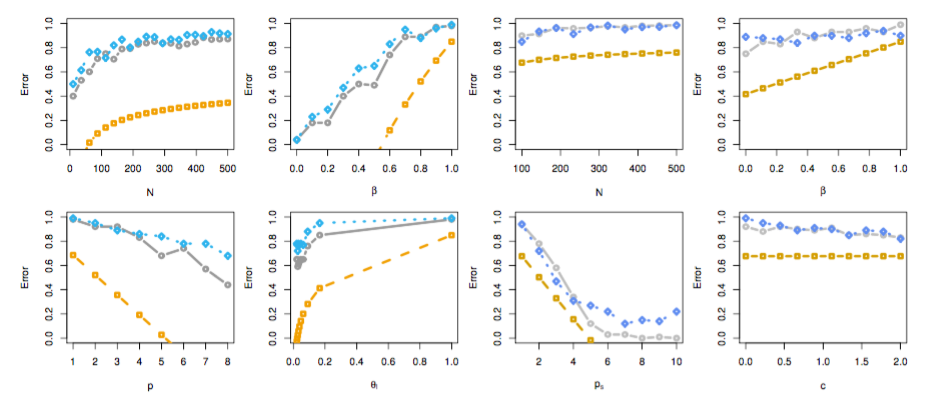
\includegraphics[width=\textwidth]{results}
%\caption{Left: Illustration when bounds are loose. Right: Illustration when bounds are tight. Gold: our method, Blue: exact matching. Grey: Gibbs sampler. }
%\label{fig:graphicalProcess}
%\end{center}
%\end{figure}
%
%
%[\textbf{RCS}, Barnes, Neiswanger (2017)]
%}
%
%\frame{
%\frametitle{Quick Takeaways}
%
%\begin{enumerate}
%\item Bayesian methods allow one to quantify the uncertainty of the entity resolution process exactly. 
%\item Since the entity resolution error can be accounted for exactly, one could then perform post-processing after
%and include the error from the entity resolution process. (See \textbf{RCS}, Hall, Fienberg (2016) for details). 
%\item We can also formalize many Bayesian models in one framework, leading to both theoretical and empirical insights for entity resolution. (See \textbf{RCS} et. al (2017) and Johndrow et al. (2017)). 
%\item Scaling is a challenge, and this is currently being explored (see \textbf{RCS} et. al (2014) and Zanella et al. (2016) for insights). 
%\end{enumerate}
%
%We now turn back to our motivating questions of interest with regard to the Syrian conflict (and other such applications). 
%
%
%}

\frame{
\frametitle{Goals of entity resolution}

Suppose that we have a total of $M$ records in $D$ data sets. 

\begin{enumerate}
\item We seek models that are much less than $O(M^2)$ (quadratic).
\item We seek models that are reliable, accurate, fit the data well, and account for the uncertainty of the model.
\end{enumerate}

\pause
These two goals fundamentally go against one another, making entity resolution a very challenging problem.
\vspace*{1em}


\pause
In order to solve the problem at hand, we will solve a slightly easier problem, where we simply provide an estimate and standard error of the number of documented identifiable deaths. 
\vspace*{1em}

\pause

We refer to this subtask of entity resolution as unique entity estimation. 

}

\frame{
\frametitle{The Linkage Graph}

\begin{figure}[htbp]
\begin{center}
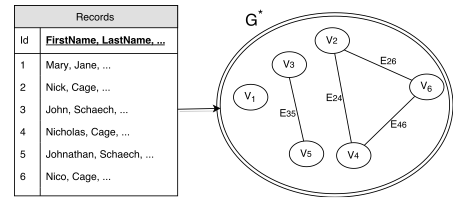
\includegraphics[width=0.8\textwidth]{figures/mapping}
\caption{Left: Records contained in $D$ datasets. Right: The unlinked data set and relationship of records viewed as a graphical model.}
\label{default}
\end{center}
\end{figure}

We don't know the edges. How do we go about estimating the probability of an edge or non-edge? 

}

\frame{
\frametitle{Desiderata} 

\begin{enumerate}
  \item The estimation cost should be significantly less than quadratic ($O(M^2)$). 
  \item To ensure accountability regarding estimating the unique number of documented identifiable victims in the Syrian conflict, it is essential to understand the statistical properties of any proposed estimator. 
  \item  In most real entity resolution tasks, duplicated data can occur with arbitrarily large changes including missing information, which we observe in the Syrian data set, and standard modeling assumptions may not hold due to the noise inherent in the data. Due to this, we prefer not to make strong modeling assumptions regarding the data generation process.
\end{enumerate}

}

\frame{
\frametitle{Related Literature: Random Sampling}
There are two methods based upon random sampling that do satisfy the above requirements, but they are sub-optimal. 
\begin{enumerate}
\item Frank (1978) proposed sampling a large enough subgraph to estimate the total number of connected components based on the properties of the sub-sampled subgraph. 
\item Chazelle, Rubinfeld, and Trevisan (2005) proposed finding connected components with high probability by sampling random vertices and then visiting their associated components using breadth-first search (BFS).
\end{enumerate}

%\begin{itemize}
%\item One major issue with random sampling is that most sampled pairs are unlikely to be matches (no edge) providing nearly no information as the underlying graph is generally very sparse in practice. 
%\item In addition, such methods often lead to a high variance of the resulting estimator. 
%\end{itemize}

}

\frame{
\frametitle{Related Literature: Random Sampling}

\begin{itemize}
\item One major issue with random sampling is that most sampled pairs are unlikely to be matches (no edge) providing nearly no information as the underlying graph is generally very sparse in practice. 
\item In addition, such methods often lead to a high variance of the resulting estimator. 
\item Finally, random sampling requires a threshold $t$ (fixed budget), which implies $t$ pairwise comparisons. 
\end{itemize}

\begin{figure}[htbp]
\begin{center}
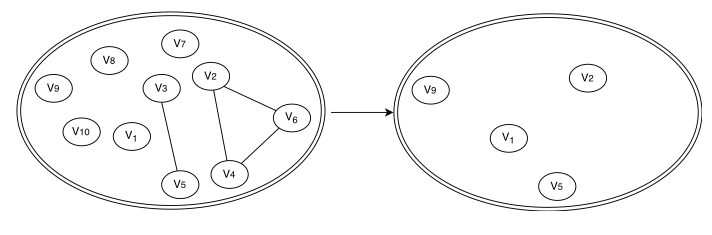
\includegraphics[width=\textwidth]{figures/random-sample}
%\caption{Left: Records contained in $D$ datasets. Right: The unlinked data set and relationship of records viewed as a graphical model.}
\label{default}
\end{center}
\end{figure}

}

%\frame{
%\frametitle{Our Goals}
%
%\begin{enumerate}
%\item {\em Our first {\bf goal} is to accurately estimate the number of unique victims.} Obtaining a match or non-match label of a given record pair may require momentous cost such as manual human supervision or involving sophisticated machine learning. 
%\item Given that coming up with hand-matched data is a costly process,  {\em our second {\bf goal}} is to provide a proxy, automated mechanism to create labeled data. 
%\end{enumerate}
%
%Chen, Shrivastava, Steorts (2017), Minor Revision, AoAS \url{https://arxiv.org/abs/1710.02690},\\
% \href{https://github.com/keroro824/RL_data/blob/master/README}{Code Link}
%
%
%}

\frame{
\frametitle{Adaptive Sampling}

\begin{itemize}
\item Here, we sample based on the similarity of the vertex pair. 
\item We assume that duplicates are likely to be similar in their textual attributes.
\item We do not assume any fixed threshold, making the method robust and computationally effient. 
\end{itemize}

Does there exist a random sampling method based on similarity with computational complexity less than sub-quadratic? 

\vspace*{1em}

Yes! (It's a variant of locality sensitive hashing (LSH). 

}

\frame{
\frametitle{Locality Sensitive Hashing (LSH)}


Hash functions are locality-sensitive if for any random hash function $h(\cdot)$ and for any pairs of data points (records) $x$ and $y$ we have the following:

\begin{enumerate}
\item Pr(h(x) = h(y)) is ``high" if x is close to y. 
\item Pr(h(x) = h(y)) is ``low" if x if far from y. 
\end{enumerate}


\begin{figure}[htbp]
\begin{center}
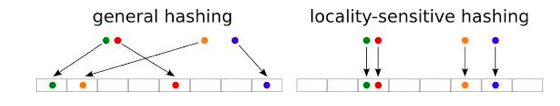
\includegraphics[width=\textwidth]{figures/lsh}
\label{default}
\end{center}
\end{figure}

As described earlier, we need to define a type of similarity and a type of dimension reduction. 

\vspace*{1em}

We will use Jaccard similarity and the minwise hash (Shrivastava and Li, 2014). 


}

\frame{
\frametitle{Our Contributions}

\begin{enumerate}
\item We formalize unique entity estimation as approximating the number of connected components in a graph with sub-quadratic $\ll O(M^2)$ computational time. 
\item We then propose a general method that provides an estimate in sample (with standard errors). 
\item Our proposal leverages locality sensitive hashing (LSH) in a novel way for the estimation process, with the required computational complexity that is less than quadratic. 
\item Our proposed estimator is unbiased and has provably low variance compared to comparable approaches in the literature. 
\item We estimate that the number of documented identifiable deaths for the Syrian conflict is 191,874, with standard deviation of 1,772, reported casualties, which is very close to the 2014 HRDAG estimate of 191,369.
% In addition, our method only takes 127s given the computationally scalability of it. 
%Our unique entity estimation procedure is broadly applicable to many applications, and we illustrate this on three additional real, fully labelled, entity resolution data sets, which include the food industry, the music industry, and an application from official statistics. In the absence of ground truth information, we estimate that the number of documented identifiable deaths for the Syrian conflict is 191,874, with standard deviation of 1,772, reported casualties, which is very close to the 2014 HRDAG estimate of 191,369. This clearly demonstrates the power of our efficient estimator in practice, which does not rely on any strong modeling assumptions. Out of 63 billion possible pairs, our estimator only queries around 450,000 adaptively sampled pairs ($\simeq O(M)$) for labels, yielding a 99.99\% reduction. The labelling was done using support vector machines (SVMs) trained on a small number of hand-matched, labeled examples provided by five domain experts. Our work is an example of the efforts required to solve a real noisy challenging problem where modeling assumptions may not hold.
\end{enumerate}

Chen, Shrivastava, \textbf{RCS} (2018), Minor Revision, AoAS \url{https://arxiv.org/abs/1710.02690},\\
 \href{https://github.com/keroro824/RL_data/blob/master/README}{Code Link}


}

\frame{
\frametitle{Notation}
\begin{itemize}
\item Let the total size of the data be $M.$ 
\item Represent the data set by a graph $G^* = (E, V).$
%\item $V_i$ corresponds to record $R_i$; vertex $V_j$ corresponds to record $R_j$.
\item Since we do not observe the edges of $G^*$ (the linkage), inferring whether there is an edge between two nodes can be costly, i.e., $O(M^2)$. 
\item Hence, one is constrained to probe a small set $\mathcal{S} \subset V \times V$ with $|\mathcal{S}|\ll O(M^2)$ of pairs and query if they have edges. 
\item The aim is to use the information about $\mathcal{S}$ to estimate the total number of connected components accurately. \item More precisely,  given the partial graph $G' = \{V,E'\}$, where $E' = E \cap \mathcal{S}$, one wishes to estimate the connected components $n$ of $G^* = \{V,E\}.$
\end{itemize}
}


\frame{
\frametitle{Unique entity estimation}

We approximate the number of connected components in the corresponding graph $G^{*},$ where the edges are not observed. 
\vspace*{2em}

\hspace{0.05\linewidth}
\center
\begin{minipage}{0.7\linewidth}
\begin{figure}[H]
			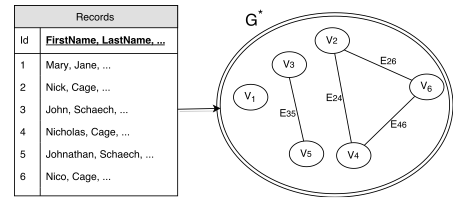
\includegraphics[width=\columnwidth]{figures/mapping}
			\caption{A toy example of mapping records to a graph, where vertices represent records and edges refer the relation between records.}
			\label{map}
\end{figure}
      \end{minipage}

}

\frame{
\frametitle{Fast Unique Entity Estimation}
\begin{enumerate}
\item Generate pairs of records using locality sensitive hashing. This places similar pairs of records into the same bin in sub-quadratic time. Output is pairs of candidate records. 
\item Query the candidate records in (1), and determine the match/non-match status either using (a) hand-matched data or (b) supervised learning algorithm. Now estimate $p$, the probability of an edge/non-edge. Next, we can form the graph $G^{'}$ from $p$ and count the number of connected components in $G^{'}$ using Breath First Search (BFS).
\item Now using the number of connected components, we can use our proposed method to estimate the number of unique entities in $G^{'}$.
\end{enumerate}

%\begin{itemize}
%\item Probe a small set of pairs of records in the sample $S$.
%\item Using ground truth records in T, we are able to infer the match status of the record pairs in $S.$ 
%\item Use information about the observed sample S to estimate the total number of connected components accurately.
%\item Using a partial graph $G^{'},$ we construct an unbiased and provably low variance estimator, which is scalable to big data.
%%\item In addition, the method is computationally scalable. 
%\end{itemize}

}

\frame{
\frametitle{Fast Unique Entity Estimation}
\begin{enumerate}
\item[1] Generate pairs of records using locality sensitive hashing (LSH). This places similar pairs of records into the same bin in sub-quadratic time. Output is pairs of candidate records. 
\end{enumerate}

We use a linear variant of LSH (Shrivastava and Li, 2014) that has been applied to entity resolution to our knowledge for the first time successfully. 
\pause
\vspace*{1em}

Why does LSH work so well?  

\begin{figure}[htbp]
\begin{center}
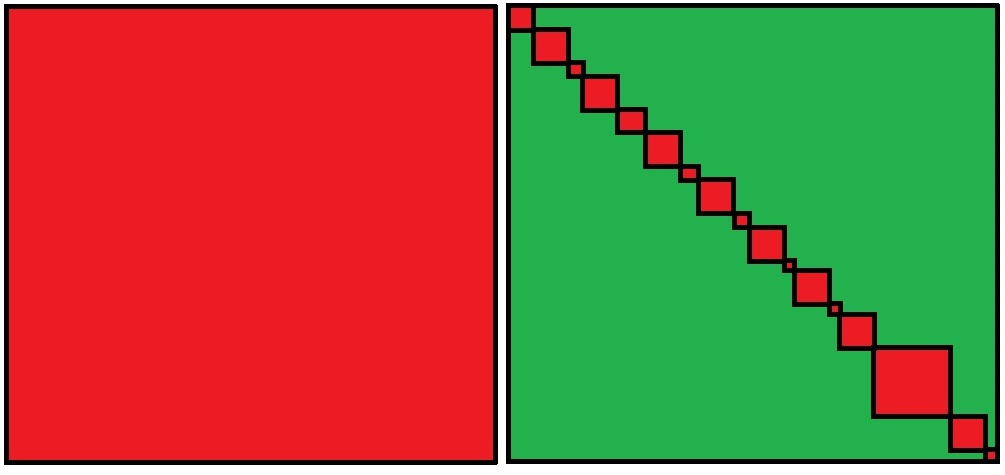
\includegraphics[width=0.5\textwidth]{figures/block}
%\caption{Not-blocking (left) versus dividing the space into partitions (left, red) and only having to run a record linkage method within each partition (right, red). }
\caption{All-to-all record comparisons (left) versus partitioning records into blocks and comparing records only within each partition (right).}
\label{block}
\end{center}
\end{figure}

%\begin{itemize}
%\item Probe a small set of pairs of records in the sample $S$.
%\item Using ground truth records in T, we are able to infer the match status of the record pairs in $S.$ 
%\item Use information about the observed sample S to estimate the total number of connected components accurately.
%\item Using a partial graph $G^{'},$ we construct an unbiased and provably low variance estimator, which is scalable to big data.
%%\item In addition, the method is computationally scalable. 
%\end{itemize}

}

\frame{
\frametitle{Fast Unique Entity Estimation}
\begin{enumerate}
%\item Generate pairs of records using locality sensitive hashing. This places similar pairs of records into the same bin in sub-quadratic time. Output is pairs of candidate records. 
\item[2] Query the candidate records in (1), and determine the match/non-match status either using (a) hand-matched data or (b) supervised learning algorithm. Now estimate $p$, the probability of an edge/non-edge. Next, we can form the graph $G^{'}$ from $p$ and count the number of connected components in $G^{'}$ using BFS.
%\item Now using the number of connected components, we can use our proposed method to estimate the number of unique entities in $G^{'}$.
\end{enumerate}

Using LSH, we reduce the record space greatly and have a new sample space $S$ of candidate records. Let $T_{match}$ represent the record  pairs in our training set that are labeled as a match. Then an unbiased estimated of $p$ (the probability that any given correct pair is sampled) is
\begin{align}
\frac{| T_{match} \cap S |}{T_{match}}.
\end{align}
Given this estimate of $p$, we can form $G^{'}$ and count the number of connected components using BFS. 

%\begin{itemize}
%\item Probe a small set of pairs of records in the sample $S$.
%\item Using ground truth records in T, we are able to infer the match status of the record pairs in $S.$ 
%\item Use information about the observed sample S to estimate the total number of connected components accurately.
%\item Using a partial graph $G^{'},$ we construct an unbiased and provably low variance estimator, which is scalable to big data.
%%\item In addition, the method is computationally scalable. 
%\end{itemize}

}

\frame{
\frametitle{Fast Unique Entity Estimation}
\begin{enumerate}
\item [3] Now using the number of connected components, we can use our proposed method to estimate the number of unique entities in $G^{'}$.
\end{enumerate}

Assuming we have an estimate of $p$, we are simply just solving the following system of equations that will map us from the unknown graph to the known graph (via $p$). 

\begin{figure}[H]
\center
	\includegraphics[width=0.6\columnwidth]{figures/p}
	\caption{A general example illustrating the transformation and probabilities of connected components from $G^*$ to $G'.$}
	\label{p}
\end{figure}


%\begin{itemize}
%\item Probe a small set of pairs of records in the sample $S$.
%\item Using ground truth records in T, we are able to infer the match status of the record pairs in $S.$ 
%\item Use information about the observed sample S to estimate the total number of connected components accurately.
%\item Using a partial graph $G^{'},$ we construct an unbiased and provably low variance estimator, which is scalable to big data.
%%\item In addition, the method is computationally scalable. 
%\end{itemize}

}

\frame{
\frametitle{Fast Unique Entity Estimation}
%\begin{enumerate}
%\item [3] Now using the number of connected components, we can use our proposed method to estimate the number of unique entities in $G^{'}$.
%\end{enumerate}

%Assuming we have an estimate of $p$, we are simply just solving the following system of equations that will map us from the unknown graph to the known graph (via $p$). 

%\begin{figure}[H]
%\center
%	\includegraphics[width=0.6\columnwidth]{fig/p.pdf}
%	\caption{A general example illustrating the transformation and probabilities of connected components from $G^*$ to $G'.$}
%	\label{p}
%\end{figure}

Let $n_i^{\prime}$ be the number of connected components of size $i$ in the observed graph G$^{\prime}.$
\vspace*{2em}

We propose an estimator and assume there exists an algorithm that adaptively samples a set of record pairs, in sub-quadratic time. 

\vspace*{2em}
Our estimator, which we call the Locality Sensitive Hashing Estimator (LSHE) for the number of connected components is given by
\begin{align}
\label{main}
\text{LSHE} &= n_1' +  n_2' \cdot \frac{2p-1}{p}  + n_3' \cdot \frac{1-6 \cdot (1-p)^2 \cdot p}{p^2 \cdot (3-2p) }
+ \sum_{i=4}^{M}n_i'.
\end{align}

It is simple to show that this estimator is unbiased and has provably low variance. 

%\begin{itemize}
%\item Probe a small set of pairs of records in the sample $S$.
%\item Using ground truth records in T, we are able to infer the match status of the record pairs in $S.$ 
%\item Use information about the observed sample S to estimate the total number of connected components accurately.
%\item Using a partial graph $G^{'},$ we construct an unbiased and provably low variance estimator, which is scalable to big data.
%%\item In addition, the method is computationally scalable. 
%\end{itemize}

}

\frame{
\frametitle{Fast Unique Entity Estimation}

\begin{figure}[htbp]
\begin{center}
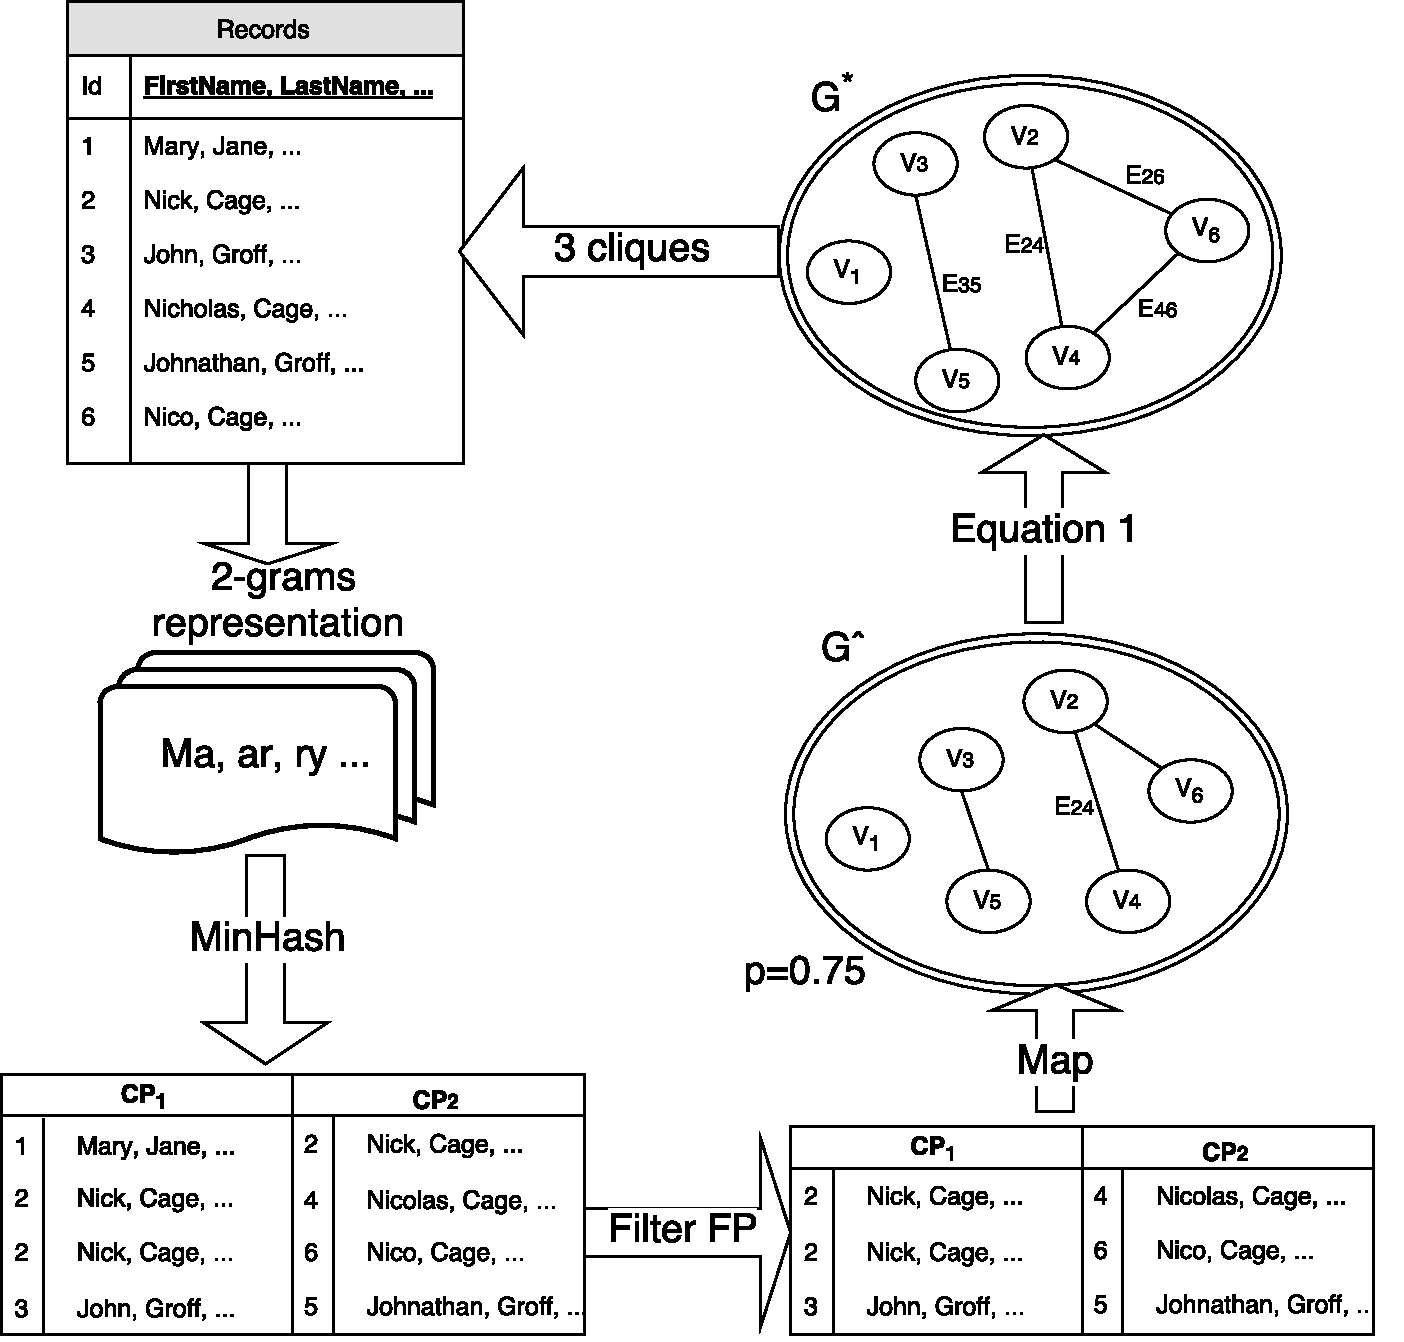
\includegraphics[width=0.7\textwidth]{figures/flow}
%\caption{default}
\label{default}
\end{center}
\end{figure}


}

%\frame{
%
%
%\begin{figure}[H]
%\center
%	\includegraphics[width=0.75\columnwidth]{fig/p.pdf}
%	\caption{A general example illustrating the transformation and probabilities of connected components from $G^*$ to $G'.$}
%	\label{p}
%\end{figure}
%
%
%}





%\frame{
%\frametitle{Our Proposal}
%
%\begin{itemize}
%\item Probe a small set of pairs of records in the sample $S$.
%\item Using ground truth records in T, we are able to infer the match status of the record pairs in $S.$ 
%\item Use information about the observed sample S to estimate the total number of connected components accurately.
%\item Using a partial graph $G^{'},$ we construct an unbiased and provably low variance estimator, which is scalable to big data.
%%\item In addition, the method is computationally scalable. 
%\end{itemize}
%
%
%
%
%
%}



%\frame{
%\frametitle{Algorithm}
%
%Input: records from a sample S, training pairs of records from T \\
%Output: An estimate of the sample size of S. 
%
%\begin{enumerate}
%\item Reduce the number of record comparison using ``locality sensitive hashing." The cost is $O(NL),$ where $L$ is a tuning parameter. 
%\item Query the reduced sample space, checking to see if pairs of records are a match or non match. The cost is $O(T).$ 
%\item The graph $G{'}$ contains edges, which are formed by the above matched pairs. We now traverse the graph, counting it's connected components, to get an estimate of the number of entities of size 1, size 2, etc. This cost is $O(N + |S|).$
%\item By requiring our estimator to be unbiased, we can now solve a system of equations, and can find our estimate.
%\end{enumerate}
%
%Similar calculations can be done for the variance. 
%
%
%}


\frame{
\frametitle{Applications}

The proposed method is applied to three real applications, with comparisons to standards in the literature. 

\begin{table}[t]
	\caption{ presents five important features of the four data sets.
%	(three well-labeled real data set and Syrian data set).
	\textbf{Domain} reflects the variety of the data type we used in the experiments. \textbf{Size} is the number of total records respectively. \textbf{\# Matching Pairs} shows how many pair of records point to the same entity in each data set. \textbf{\# Attributes} represents the dimensionality of individual record. \textbf{\# Entities} is the number of unique records.}
	\label{table1}
	\centering
	\tiny
				
	\begin{tabular}{lccccc}
		\toprule
		\textbf{DBname} & \textbf{Domain}& \textbf{Size} & \textbf{\# Matching Pairs} & \textbf{\# Attributes}& \textbf{\# Entities} \\
		\midrule
		Restaurants & Restaurant Guide&864  &112 & 4&752 \\
	
		CD & Music CDs&9,763  &299 & 106 & 9,508\\
	
		Voter & Registration Info&324,074  & 70,359 & 6 & 255,447\\
	
		Syria & Death Records&296,245  & N/A & 7 & N/A\\
		\bottomrule
	\end{tabular}	
\end{table}


}

%\begin{table}[t]
%	\caption{ shows part of the sample sizes (in \% in TOTAL) for different set of samples generated by Min-Wise Hashing and their corresponding $p$ in all three data sets.}
%	\label{table2}
%	\centering
%	\setlength\tabcolsep{0.18cm}
%		\begin{tabular}{l|cccc|cccc|cccc}
%			\toprule
%			\multicolumn{4}{c}{\textbf{Restaurant}}&\multicolumn{4}{c}{\textbf{CD}}&\multicolumn{4}{c}{\textbf{Voter}}
%			\\
%			\midrule
%			Size&1.0&2.5&5.0&10&0.005 & 0.01& 0.02 & 0.04&0.002&0.006&0.009&0.013
%			\\
%			
%			$p$&0.42&0.54&0.65&0.82& 0.72& 0.74& 0.82& 0.92& 0.62&0.72& 0.76& 0.82
%			\\
%			\bottomrule
%		\end{tabular}
%	\vskip -0.1in
%\end{table}

%\frame{
%\frametitle{Comparisons}
%Our method is denoted by the LSH based Estimator (LSHE). We compare to the following methods: 
%
%\begin{itemize}
%\item We consider the non-adaptive variant of our estimator (PRSE), where the sampling is plain random sampling (instead of adaptive). This baseline quantifies the advantages of proposed adaptive sampling over random sampling. 
%\item We consider the tranditional sampling methods proposed in \cite{1978paper} and \cite{chazelle2005approximating}, denoting them as Random Sub-Graph based Estimator (RSGE), and BFS on Random Vertex based Estimator (BFSE) respectively.
%\end{itemize}
%
%In addition, we compute the relative error ($RE$) of our estimates for different sample sizes, where $RE = \dfrac{|Est - n|}{n}.$
%
%
%
%}

\frame{
\frametitle{Results}

\begin{figure}[htbp]
\begin{center}
\includegraphics[width=0.7\textwidth]{figures/restaurant}
%\caption{In its third report on Syria commissioned by the United Nations, the Human Rights Data Analysis Group identified 191,369 deaths from the start of the conflict in March 2011 to April 2014, more than double the 92,901 deaths cited in the group?s last report, which covered the first two years of the conflict.}
\label{default}
\end{center}
\end{figure}

\begin{itemize}
\item Our methods: Red (LSHE) and black (LSHE + SVM) 
\item Comparisons: blue and green (random sampling)
\end{itemize}


}

\frame{
\frametitle{Results}

\begin{figure}[htbp]
\begin{center}
\includegraphics[width=0.7\textwidth]{figures/cd}
%\caption{In its third report on Syria commissioned by the United Nations, the Human Rights Data Analysis Group identified 191,369 deaths from the start of the conflict in March 2011 to April 2014, more than double the 92,901 deaths cited in the group?s last report, which covered the first two years of the conflict.}
\label{default}
\end{center}
\end{figure}

\begin{itemize}
\item Our methods: Red (LSHE) and black (LSHE + SVM) 
\item Comparisons: blue and green (random sampling)
\end{itemize}


}

\frame{
\frametitle{Results}

\begin{figure}[htbp]
\begin{center}
\includegraphics[width=0.7\textwidth]{figures/voter}
%\caption{In its third report on Syria commissioned by the United Nations, the Human Rights Data Analysis Group identified 191,369 deaths from the start of the conflict in March 2011 to April 2014, more than double the 92,901 deaths cited in the group?s last report, which covered the first two years of the conflict.}
\label{default}
\end{center}
\end{figure}

\begin{itemize}
\item Our methods: Red (LSHE) and black (LSHE + SVM) 
\item Comparisons: blue and green (random sampling)
\end{itemize}


}




%\frame{
%\frametitle{Results}
%
%
%
%\begin{figure}[H]
%%\begin{figure}[!Htb]
%	%	\centering
%	\mbox{
%		\hspace{-0.1in}
%		\includegraphics[width=.36\linewidth]{fig/restaurant}\hspace{-0.18in}
%		\includegraphics[width=.36\linewidth]{fig/cd}\hspace{-0.16in}
%		\includegraphics[width=.36\linewidth]{fig/voter}}
%%	\caption{ The dashed lines show the $\text{RE}$ of the four estimators on the three real data sets, where the y-axis is on the log-scale. Observe that LSHE outperforms all other three estimators in one to two orders of magnitude. The standard deviation of the $\text{RE}$ for LSHE is also shown in the plots with the red error bars, which is with respect to randomization of hash functions.  In particular, the PRSE performs unreliable estimation on the CD and Voter data sets. The dashed and solid black lines represent RE of LSHE using ground truth labels and a SVM classifier.}
%	\label{fg1}
%\end{figure}
%
%
%
%
%
%}
%
%\frame{
%\frametitle{Results}
%
%\begin{figure}[H]
%%\begin{figure}[!Htb]
%	%	\centering
%	\mbox{
%		\hspace{-0.1in}
%		\includegraphics[width=.36\linewidth]{fig/restaurant}\hspace{-0.18in}
%		\includegraphics[width=.36\linewidth]{fig/cd}\hspace{-0.16in}
%		\includegraphics[width=.36\linewidth]{fig/voter}}
%	\caption{ The dashed lines show the $\text{RE}$ of the four estimators on the three real data sets, where the y-axis is on the log-scale. Observe that LSHE outperforms all other three estimators in one to two orders of magnitude. The standard deviation of the $\text{RE}$ for LSHE is also shown in the plots with the red error bars, which is with respect to randomization of hash functions.  In particular, the PRSE performs unreliable estimation on the CD and Voter data sets. The dashed and solid black lines represent RE of LSHE using ground truth labels and a SVM classifier.}
%	\label{fg1}
%\end{figure}
%
%
%
%
%
%}


%\frame{
%\frametitle{Results}
%
%
%\begin{figure}[H]
%%\begin{figure}[!Htb]
%	%	\centering
%	\mbox{
%		\hspace{-0.1in}
%		\includegraphics[width=.36\linewidth]{fig/restaurant_1.pdf}\hspace{-0.18in}
%		\includegraphics[width=.36\linewidth]{fig/CD_1.pdf}\hspace{-0.16in}
%		\includegraphics[width=.36\linewidth]{fig/voter_1.pdf}}
%	\caption{ The dashed lines show the RE of four estimators on three data sets. It can be observed that LSHE outperforms all the other three estimators in one to two order of magnitude. Particularly, PRSE performs unreliable estimation on CD and Voter data set. The dashed and solid black lines represent RE of LSHE using ground truth labels and a simple support vector machine (y-axis is in log scale).}
%	\label{fg1}
%\end{figure}
%
%
%}

%\frame{
%\frametitle{Syrian Data --- Documented, Identifiable Victims}
%
%What resources we have:
%	\begin{itemize}
%	\item Human Rights Data Analysis Group collects 300,000 death records from Syria.
%\item Records reported from four human rights groups in Syria (March 2011 --- November 2014).  
%\item Field attributes: Full Arabic name, date of death (DOD), governorate, other less reliable ones. 
%%		\item Large number of record pairs labeled as match/non-match.
%		\item 200,000+ record pairs labeled as match/non-match (but biased).
%	\end{itemize}
%
%
%}



\frame{
\frametitle{Application to Syrian Conflict}
One main challenge with Syria is that the hand-labeled data is biased. 
A major goal is to also use this method for an automated labeling process. 

\begin{itemize}
\item Since we have a reasonable size of manually labeled pairs, we train a support vector machine based upon these pairs, where we split data into a training and test set. 
\item We verify the labeling accuracy of the SVM's on the test set.
\item We believe this to be reasonable given the accuracy on approaches for the three real data sets considered earlier. 
\item That is, when ground truth is noisy or biased, this method can be used as a proxy for ground truth measurements. 
\end{itemize}

}



\frame{
\frametitle{Evaluation Methods}
\begin{enumerate}
\item  Pairs of data can be linked in both the handmatched
training data (which we refer to as ``truth") and under the estimated
linked data. We refer to this situation as true positives (TP). 
\item Pairs of data can be linked under the truth but not linked under the estimate, which
are called false negatives (FN). 
\item Pairs of data can be not linked under the truth but linked under the estimate, which are called false positives (FP). 
\item  Pairs of data can be not linked under the truth and also not linked
under the estimate, which we refer to as true negatives (TN).
\end{enumerate}


}


\frame{
\frametitle{Recall, Precision, Reduction Ratio}

$$\text{Recall} = \frac{TP}{TP + FN} = 1 - FNR.$$\\
\pause
$$\text{Precision} = \frac{TP}{TP + FP} = 1 - FPR.$$\\

\pause

\vspace{1em}

Reduction ratio (RR) measures the relative reduction of the comparison space from the de-duplication or hashing technique. 

\vspace*{1em}

See Christen (2012), Steorts, Ventura, Sadinle, Fienberg (2014) for a formal definition. 

}






\frame{
\frametitle{Final Estimate}

\begin{itemize}
\item Using our proposed methodology, used 917,577 sampled pairs and then used an SVM for classification of matches and non-matches. 
\item After looking at a sensitivity analysis of the tuning parameters for our proposed method, we report that there are 191,874 documented identifiable deaths, with standard deviation of 1,772, which is very close to HRDAG's estimate of 191,369 in Price et al. (2014).
\item Furthermore, we also report the recall (false positives) = 0.83 and the precision (false negatives) = 0.99. 
\item Finally, one iteration of the method takes only 127 seconds! (Real time estimation is possible). 
\end{itemize}
}





%\frame{
%\frametitle{Reduction Ratio versus Recall}
%
%
%
%
%}




\frame{
\center

Questions? beka@stat.duke.edu

\vspace*{1em}

Thank you to Patrick Ball and Megan Price at the Human Rights Data Analysis Group for providing the data and for fruitful conversations that have 
constantly improved the work. This work would not have been possible without the encouragement and mentorship of Steve Fienberg.\\

\vspace*{1em}

Thank you to the National Science Foundation for NSF CAREER Microclustering and NSF Big Data Privacy. The views in this talk are of the authors alone and not of the funding organization. 


}

\frame{
%\pause
%$$RR = 1 - \frac{s_M + s_N}{n_M+n_N}.$$ 
%
%\begin{itemize}
%% without assessing the quality of these candidate record pairs.
%\item $n_M$ and $n_N$ are the total of matched and non-matched records.
%\item The number of true matched and true non-matched candidate record pairs generated by an indexing technique is denoted with
%$s_M + s_N \leq n_M+n_N.$ 
%\end{itemize}

\begin{figure}[htbp]
\begin{center}
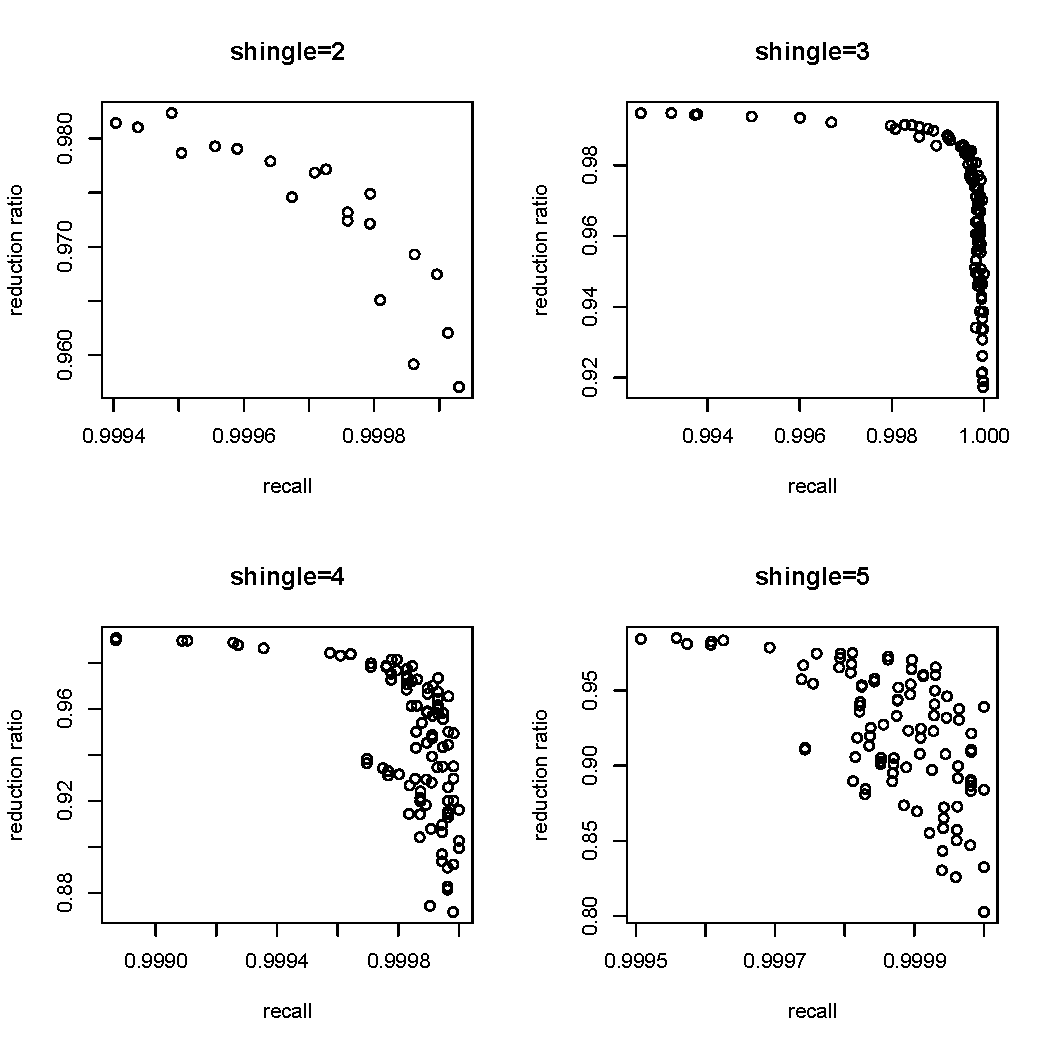
\includegraphics[width=0.65\textwidth]{figures/syria_full_recall_rr_allShingles}
%\caption{For shingles 2--5, we plot the RR versus the recall. Overall, we see the best behavior for a shingle of 3, where the RR and recall can be reached at 0.98 and 1, respectively. We allow L and K to vary on a grid here. L varies from 5--100 by steps of 5; and K takes values 15, 18, 20, 23, 25, 28, 30, 32, and 35.}
%\label{syria-takethatAssad}
\end{center}
\end{figure}


}



%%% BEGIN BACK UP SLIDES   %%%%
\beginbackup
\appendix

\frame{
\frametitle{What is a hash function?}

Find a hash function $h()$ such that
\begin{itemize}
\item if $\text{sim}(A,B)$ is high, then with high prob.\ $h(A) = h(B).$
\item if $\text{sim}(A,B)$ is low, then with high prob.\ $h(A) \neq h(B).$
\end{itemize}
%\pause
%\begin{itemize}
%\item The hash function depends on the similarity metric.
%\item Not all similarity metrics have a suitable 
%hash function.
%\item The hash function for the Jaccard similarity is min-hashing.


}

\begin{frame}
\frametitle{Locality-Sensitive Hashing}
\begin{itemize}
\item LSH tries to preserve similarity after dimension reduction.
\begin{itemize}
\item What kind of similarity? $\leftrightarrow$ What kind of dimension reduction?
\end{itemize}
%\item Euclidean inner product of vectors $\leftrightarrow$ Linear projection of vectors.
%\item Jaccard similarity (relative intersection) of sets $\leftrightarrow$ ``minhash" of sets.
%\item Could use either, if we turn records into sets or into vectors.
%\item Neither gives probability of a match.
%\begin{itemize}
%\item Both are useful and fast to find.
%\end{itemize}
\end{itemize}
\end{frame}


%\frame{
%\frametitle{Variational Bayes and Record Linkage}
%Take the methods of \textcolor{blue}{Steorts} et al.\ (2014a,b), \textcolor{blue}{Steorts} (2014).
%\begin{enumerate}
%
%\item Find a close generative model for these that looks like Latent Dirichlet Allocation (LDA). \textcolor{blue}{\checkmark}
%\item Find a mean-field variational Bayesian (VB) approximation. \textcolor{blue}{ \checkmark}
%\item Find that the VB approximation has issues with local maxima. 
%\item Possible solutions?
%%\item Using simulated and real data, see how close the VB approximation is to the LDA-like model.
%\end{enumerate}
%\begin{flushright}
%[Broderick and \textcolor{blue}{Steorts} (2014), \emph{Advances in Variational Inference}, NIPS Workshop 2014; In Preparation Paper for NIPS 2015]
%
%\end{flushright}
%}

\frame{
\frametitle{Empirical Bayes Model }
\small
\begin{itemize}
\item Define
$
\alpha_\ell(w)=
%\frac{1}{N}\sum_{i=1}^k\sum_{j=1}^{n_i}I(X_{ij\ell}=w).%=
\text{relative frequency of $w$ in data for field $\ell$}.
$
\pause
\item $G_\ell$: empirical distribution for field $\ell.$
%\item $W \sim G_\ell, \implies \forall w$,
%$
%P(W=w)=\alpha_\ell(w).
%$
\pause
\item $W\sim F_\ell(w_0)$: $\textcolor{black}{P(W=w)\propto\alpha_\ell(w)\,\exp\!\left[-c\,d(w,w_0)\right],}$
where $d(\cdot,\cdot)$ is a string metric and $c>0$.
\end{itemize}
\pause
\vspace*{-1em}
\begin{align*}
X_{ij\ell}\mid \lambda_{ij},\,Y_{\lambda_{ij}\ell},\,z_{ij\ell}\;&\sim\begin{cases}\delta(Y_{\lambda_{ij}\ell})&\text{ if }z_{ij\ell}=0\\F_\ell(Y_{\lambda_{ij}\ell})&\text{ if }z_{ij\ell}=1\text{ and field }\ell\text{ is string-valued}\\G_\ell&\text{ if }z_{ij\ell}=1\text{ and field }\ell\text{ is categorical}\end{cases}\\
%&\qquad\text{for each }i\in\{1,\ldots,k\},\; j\in\{1,\ldots,n_i\},\; \ell\in\{1,\ldots,p_s+p_c\},\\
%&\qquad\text{with everything independent},\\
Y_{j'\ell}\;&\sim G_\ell\\
z_{ij\ell}\mid\beta_{i\ell}\;&\sim \text{Bernoulli}(\beta_{i\ell})\\
\beta_{i\ell}\;&\sim\text{Beta}(a,b)\\
\lambda_{ij}\;&\sim\text{DiscreteUniform}(1,\ldots,N_{\max}),\quad
\text{ where }N_{\max}=\sum_{i=1}^k n_i.
\end{align*}
%with everything independent of everything else.


}


\frame{
\frametitle{Why Bayesian?}

\begin{enumerate}
\item Latent entity for clustering allows us to handle many databases.
\item Method is general to many applications.
\item Scalability for categorical data is quite good. 
\item We can provide a summary of the linkages using what we call the shared most probable maximal matching set. 
\item The linkage structure is flexible -- provides more than just links/non-links. 
%Full posterior, posterior standard errors, post analyses possible. 

\end{enumerate}
}

\frame{
\frametitle{Error Propagation for Estimating Death Counts}

$$Var(N \mid \bX) = Var_{\lam \mid \bX} E[ N \mid \lam]$$

\pause

This estimate is only as good as the model that we are fitting! 





}

\frame{
\frametitle{Total Variance Decomposition}

\begin{align}
Var(N \mid \bX) &= Var_{\lam \mid \bX} E[ N \mid \lam] \\
&= E_{\lam \mid \bX} \left \{
Var_{m \mid \lam} E[ N \mid \lam, m] 
\right \} \\
&+
E_{\lam \mid \bX} \left\{
E_{m \mid \lam} Var[ N \mid \lam, m] 
\right \} 
\end{align}


}

\frame{
\frametitle{Population sized estimation}

\begin{itemize}
\item Target: size $N$ of a population (not sample).
\end{itemize}

\begin{figure}[htbp]
\begin{center}
\includegraphics[width=0.7\textwidth]{figures/population}
%\caption{default}
\label{default}
\end{center}
\end{figure}

\begin{itemize}
\item From these capture histories we can find $p_A(N \mid \boldsymbol{n}).$
\end{itemize}


}

%\frame{
%\frametitle{Population sized estimation}
%
%\begin{itemize}
%\item Target: size $N$ of a population (not sample).
%\end{itemize}
%
%\begin{figure}[htbp]
%\begin{center}
%\includegraphics[width=0.7\textwidth]{population}
%%\caption{default}
%\label{default}
%\end{center}
%\end{figure}
%
%\begin{itemize}
%\item From these capture histories we can find $p_A(N \mid \boldsymbol{n}).$
%\end{itemize}
%
%
%}

\frame{
\frametitle{Population sized estimation}

Uncertainty in $\lam$ is captured by $p_L(\lam \mid \bX).$

\begin{align*}
p_C(N\mid \bX) \propto \sum_{\lam} \text{linkage model likelihood} & \times p(N, \lam) \\
=  \sum_{\lam} \text{linkage model likelihood} &\times p_A(N \mid \bm{n}) p (\lam).
\end{align*}


}


%\begin{frame}[fragile]
%\frametitle{Shingles, Tokens, Grams}
%Turn records into sets and vectors ("shingles", "tokens", ``grams"):
%\begin{itemize}
%\item Look at all length-$k$ substrings of a record ($k$-grams).
%\item Represent the record by its set of $k$-grams.
%%\item Or look at the "bag of $k$-grams" vector, with counts
%\end{itemize}
%
%\pause
%{\scriptsize
%\begin{verbatim}
%> table(tokenify("david davies",k=2))
% d av d  da es id ie vi 
% 1  2  1  2  1  1  1  2 
% 
%\end{verbatim}
%\end{frame}


%\frame{
%\frametitle{Densified One Permutation Hashing}
%
%Proposed by  Shrivastava and Li (2014). 
%
%\begin{itemize}
%\item Instead of minhashing, we use b-bit minhasing. 
%\item That is, we store the lowest b-bits. 
%\item  We can use just one permutation, break the space
%evenly into $k$ bins, and store the smallest nonzero in each bin. 
%\item The new hash function is a rotation scheme which densifies the sparse sketches of one permutation hashing  in an unbiased way and preserves the LSH property.
%
%
%
%\end{itemize}
%
%\begin{figure}[htbp]
%\begin{center}
%\includegraphics[width=0.7\textwidth]{one-permutation}
%%\caption{default}
%\label{default}
%\end{center}
%\end{figure}
%
%
%}




\backupend

\end{document}